% ---------------------------------------------------------------------------
% HOPPER v8 — Technical Whitepaper
% Build: tectonic hopper-whitepaper.tex
% ---------------------------------------------------------------------------
\documentclass[11pt,a4paper]{article}

\usepackage[a4paper,top=24mm,bottom=26mm,left=24mm,right=24mm,headheight=21pt]{geometry}

\usepackage{fontspec}
\setmainfont{Liberation Serif}
\setsansfont{Liberation Sans}
\setmonofont{DejaVu Sans Mono}[Scale=0.78]
\usepackage{newtxmath}
\usepackage{amsmath}

\usepackage{microtype}
\usepackage[table]{xcolor}
\usepackage{graphicx}
\usepackage{booktabs,tabularx,array,multirow}
\usepackage{float}
\usepackage{enumitem}
\usepackage{caption}
\usepackage{listings}
\usepackage{algorithm}
\usepackage{algpseudocode}
\usepackage{tcolorbox}
\tcbuselibrary{breakable,skins}
\usepackage{tikz}
\usetikzlibrary{arrows.meta,positioning,calc,fit,backgrounds,shapes.geometric}
\usepackage{pgfplots}
\pgfplotsset{compat=1.18}
\usepackage{fancyhdr}
\usepackage{titlesec}
\usepackage[hidelinks]{hyperref}
\usepackage{xurl}

\definecolor{ink}{HTML}{1B2A1F}
\definecolor{deepgreen}{HTML}{1E3A28}
\definecolor{midgreen}{HTML}{3F6B4A}
\definecolor{accent}{HTML}{C9A227}
\definecolor{accentlight}{HTML}{E8D48B}
\definecolor{paper}{HTML}{FBF9F2}
\definecolor{pale}{HTML}{EEF2E9}
\definecolor{muted}{HTML}{6E7A6C}
\definecolor{deadred}{HTML}{8C3B32}
\definecolor{codebg}{HTML}{F4F5EE}

\hypersetup{
  pdftitle={HOPPER: A Satoshi-Native Game Protocol on Bitcoin},
  pdfauthor={The HOPPER contributors},
  pdfsubject={HOPPER v8 protocol, wire version 0x08},
  pdfkeywords={Bitcoin, ordinals, inscriptions, Taproot, tapscript, protocol, PWA},
  colorlinks=true,
  linkcolor=deepgreen,
  citecolor=deepgreen,
  urlcolor=midgreen,
  pdfcreator={XeTeX / Tectonic}
}

\linespread{1.035}
\setlength{\parindent}{1.15em}
\setlength{\parskip}{0.18em}
\setlength{\emergencystretch}{2.5em}
\clubpenalty=10000
\widowpenalty=10000

% ---------------------------------------------------------------------------
% Macros
% ---------------------------------------------------------------------------
\newcommand{\code}[1]{\texttt{\detokenize{#1}}}
\newcommand{\term}[1]{\textbf{#1}}
\newcommand{\SHA}{\operatorname{SHA256}}
\newcommand{\LE}{\operatorname{LE}}
\newcommand{\floor}[1]{\left\lfloor #1 \right\rfloor}
% The road mark used by the live band (U+1F6E3 in the implementation).
\newcommand{\roadglyph}{\raisebox{0.08ex}{\tikz[baseline=0pt]{
  \fill[midgreen] (0,0) rectangle (0.52em,0.10em);
  \fill[midgreen] (0.06em,-0.16em) rectangle (0.46em,-0.06em);}}}
\newcommand{\nameband}[1]{\texttt{NAME}\roadglyph\texttt{#1}}

% ---------------------------------------------------------------------------
% Section styling
% ---------------------------------------------------------------------------
\titleformat{\section}
  {\sffamily\Large\bfseries\color{deepgreen}}
  {\thesection}{0.72em}{}
  [\vspace{0.35ex}{\color{accent}\titlerule[0.6pt]}]
\titleformat{\subsection}
  {\sffamily\large\bfseries\color{midgreen}}
  {\thesubsection}{0.65em}{}
\titleformat{\subsubsection}
  {\sffamily\normalsize\bfseries\color{ink}}
  {\thesubsubsection}{0.6em}{}
\titlespacing*{\section}{0pt}{2.5ex plus .5ex minus .15ex}{1.1ex}
\titlespacing*{\subsection}{0pt}{1.8ex plus .3ex minus .1ex}{0.6ex}
\titlespacing*{\subsubsection}{0pt}{1.3ex plus .2ex}{0.4ex}

% ---------------------------------------------------------------------------
% Header and footer
% ---------------------------------------------------------------------------
\pagestyle{fancy}
\fancyhf{}
\fancyhead[L]{\sffamily\scriptsize\color{muted}HOPPER \textperiodcentered{} Technical Whitepaper}
\fancyhead[R]{\sffamily\scriptsize\color{muted}v8 \textperiodcentered{} wire 0x08}
\fancyfoot[C]{\sffamily\scriptsize\color{muted}\thepage}
\renewcommand{\headrulewidth}{0.25pt}
\renewcommand{\headrule}{\hbox to\headwidth{\color{accentlight}\leaders\hrule height \headrulewidth\hfill}}
\fancypagestyle{plain}{%
  \fancyhf{}%
  \fancyfoot[C]{\sffamily\scriptsize\color{muted}\thepage}%
  \renewcommand{\headrulewidth}{0pt}%
}

% ---------------------------------------------------------------------------
% Captions
% ---------------------------------------------------------------------------
\captionsetup{
  font=small,
  labelfont={bf,sf,color=deepgreen},
  textfont={it},
  justification=raggedright,
  singlelinecheck=false,
  skip=6pt
}

% ---------------------------------------------------------------------------
% Boxes
% ---------------------------------------------------------------------------
\newtcolorbox{notebox}{
  enhanced, breakable,
  colback=pale, colframe=pale, boxrule=0pt,
  left=5mm, right=5mm, top=3.2mm, bottom=3.2mm,
  arc=0pt, outer arc=0pt,
  borderline west={1.2pt}{0pt}{accent}
}
\newtcolorbox{invariant}[1]{
  enhanced, breakable,
  colback=deepgreen!4, colframe=deepgreen!18, boxrule=0.4pt,
  left=5mm, right=5mm, top=2.6mm, bottom=2.8mm,
  arc=0pt, outer arc=0pt,
  title={\sffamily\bfseries\small #1},
  coltitle=white, colbacktitle=deepgreen,
  fonttitle=\sffamily\bfseries\small
}
\newtcolorbox{warnbox}[1]{
  enhanced, breakable,
  colback=deadred!4, colframe=deadred!22, boxrule=0.4pt,
  left=5mm, right=5mm, top=2.6mm, bottom=2.8mm,
  arc=0pt, outer arc=0pt,
  title={\sffamily\bfseries\small #1},
  coltitle=white, colbacktitle=deadred,
  fonttitle=\sffamily\bfseries\small
}

% ---------------------------------------------------------------------------
% Listings
% ---------------------------------------------------------------------------
\lstdefinestyle{hopper}{
  backgroundcolor=\color{codebg},
  basicstyle=\ttfamily\footnotesize,
  keywordstyle=\color{deepgreen}\bfseries,
  commentstyle=\color{muted}\itshape,
  stringstyle=\color{deadred},
  numbers=left,
  numberstyle=\ttfamily\scriptsize\color{muted},
  numbersep=8pt,
  frame=none,
  breaklines=true,
  columns=fullflexible,
  keepspaces=true,
  showstringspaces=false,
  tabsize=2,
  xleftmargin=15pt,
  framexleftmargin=0pt,
  aboveskip=8pt,
  belowskip=7pt,
  upquote=true
}
\lstset{style=hopper}

% ---------------------------------------------------------------------------
% Algorithm styling
% ---------------------------------------------------------------------------
\algrenewcommand\algorithmicrequire{\textbf{Input:}}
\algrenewcommand\algorithmicensure{\textbf{Output:}}
\algrenewcommand\algorithmicwhile{\textbf{while}}
\algrenewcommand\algorithmicfor{\textbf{for}}
\algrenewcommand\algorithmicif{\textbf{if}}
\algrenewcommand\algorithmicthen{\textbf{then}}
\algrenewcommand\algorithmicelse{\textbf{else}}
\algrenewcommand\algorithmicreturn{\textbf{return}}
\floatname{algorithm}{Algorithm}
\renewcommand{\listalgorithmname}{List of Algorithms}

\begin{document}

% ---------------------------------------------------------------------------
% Front matter: cover, abstract, contents
% ---------------------------------------------------------------------------
\begin{titlepage}
\thispagestyle{empty}
\begin{tikzpicture}[remember picture,overlay]
  \fill[paper] (current page.north west) rectangle (current page.south east);
  \fill[deepgreen] (current page.north west) rectangle ([yshift=-8mm]current page.north east);
  \fill[accent] ([yshift=-8mm]current page.north west) rectangle ([yshift=-9mm]current page.north east);
  % faint pixel rule at the foot
  \fill[accentlight!55] ([yshift=16mm]current page.south west) rectangle ([yshift=16.4mm]current page.south east);
\end{tikzpicture}

\vspace*{12mm}
{\sffamily\scriptsize\color{muted}\MakeUppercase{Hopper Protocol}\hfill Technical Whitepaper}
\vspace{2mm}

\vspace{14mm}
\begin{center}
  
\includegraphics[width=46mm]{figures/hopper-logo.png}\\[10mm]
  {\sffamily\bfseries\color{deepgreen}\fontsize{60}{64}\selectfont HOPPER}\\[3mm]
  {\sffamily\Large\color{ink} A Satoshi-Native Game Protocol\\[1.2mm] on Bitcoin}\\[9mm]
  {\color{accent}\rule{54mm}{1.1pt}}\\[7mm]
  {\large\itshape One satoshi. One life.\\[1mm] The chain is the referee.}
\end{center}

\vfill
\begin{center}
  \begin{tabular}{@{}c@{}}
    {\sffamily\small\color{deepgreen}\textbf{Wire version} \code{0x08}}\\[1.2mm]
    {\sffamily\small\color{muted}Specification 3.0 \textperiodcentered{} October 2026}\\[1.2mm]
    {\sffamily\small\color{muted}The HOPPER contributors}
  \end{tabular}
\end{center}
\vspace*{10mm}
\end{titlepage}

% ---------------------------------------------------------------------------
% Abstract
% ---------------------------------------------------------------------------
\pagenumbering{roman}
\thispagestyle{plain}
\section*{Abstract}
\addcontentsline{toc}{section}{Abstract}

\begin{notebox}
\noindent
HOPPER is a game played by a satoshi. A frog is an ordinal sat whose public
life is written into Bitcoin itself: a mint inscription creates it, each
crossing publishes a 55-byte state inscription on the same sat, and the
direction carried in that inscription is judged against the one direction
the next block wraps to. Custody is enforced by a four-leaf Taproot output
with a nothing-up-my-sleeve internal key. Three crossing leaves, one per
direction, each check the owner's signature and carry the protocol envelope;
the fourth leaf is an ordinary owner signature for transfers. The v8 fold
verifies every crossing body against the raw transaction that published it;
if a proof is missing, the art says so rather than guessing. The road's
difficulty runs in generations: it rises from five crossings to a ceiling of
twenty-five and then resets. One released v7 Hopper is grandfathered for
custody and play. No server signs, no external origin is needed to render the
frog, and the indexer is a cache, not an authority.

This paper specifies the wire format, the generation schedule, the
block-wide wrap, the tapscript tree and transaction shapes that play the
game, and the standalone indexer and JavaScript wallet that implement them.
It is an exposition of the normative specification in \code{SPEC.md}; where
the two documents differ, \code{SPEC.md} governs.
\end{notebox}

\vspace{4mm}
\noindent\textbf{\sffamily Keywords:} Bitcoin, ordinals, inscriptions,
Taproot, tapscript, ordinal theory, self-custody, PWA.

\vspace{2mm}
\noindent\textbf{\sffamily Normative source.} The repository specification
\code{hopper-protocol/SPEC.md} is the single normative source for the
consensus rules, byte layouts, constants, API surface and configuration
described here. Code snippets are illustrative; byte strings, constants and
acceptance conditions are quoted from that document.

\vspace{6mm}
{\small\color{muted}\noindent
The historical mint magic \code{FRG} and the JSON keys
\code{frog}/\code{frogger} are retained because they are already committed to
Bitcoin. The current state magic is \code{FRG8CROSS}; the legacy
\code{FRG7CROSS} is accepted only for the one grandfathered Hopper. The
interface name is \textsf{HOPPER}; the crossing action is \code{HOP} in the
interface and \code{cross} on the wire.}

\clearpage

% ---------------------------------------------------------------------------
% Contents
% ---------------------------------------------------------------------------
\thispagestyle{plain}
\renewcommand{\contentsname}{\sffamily\color{deepgreen}Contents}
\tableofcontents
\vfill
\begin{notebox}
\small
\textbf{Reading guide.} Sections~\ref{sec:parameters}--\ref{sec:custody}
are the consensus core. Sections~\ref{sec:indexer} and~\ref{sec:wallet}
describe infrastructure that can be replaced without changing the protocol.
Section~\ref{sec:security} states what the construction does and does not
protect against.
\end{notebox}
\clearpage


\pagenumbering{arabic}

\section{Introduction}\label{sec:introduction}

Bitcoin \cite{bitcoin} is usually described as a ledger of coins. Ordinal theory gives that
ledger a second reading: every satoshi has a number, sats move through
transactions in first-in-first-out order, and a particular sat can therefore
be followed across the chain. HOPPER uses that identity directly. A frog is
not a token contract, a database row, or an entry in a server's table. A frog
is one satoshi, and its public life is the sequence of transactions that
carry that satoshi.

The game is small enough to state in one paragraph. A player mints a frog by
inscribing a self-contained art document on a sat. A one-time \textsc{prepare}
may move the frog from its mint output into the custody output. To move the
frog forward, the owner spends the sat through one of three Taproot leaves and
publishes a 55-byte state inscription naming the direction it picked: left,
straight or right. The crossing confirms at height $T$. At block $T+1$ the
block hash wraps to exactly one direction for the whole block, and every
frog whose crossing confirmed in $T$ that picked that direction dies at
$T+\kappa$. A frog that survives enough crossings reaches \emph{home} and
becomes immortal. A plain transfer moves the sat without publishing anything
and without changing the frog's state. The chain is the referee, and the
owner chooses \emph{when} to hop and \emph{which way}, never whether the road
agrees.

\subsection{Design goals}

The construction is organized around four goals.

\begin{description}[leftmargin=1.4em,style=nextline,itemsep=0.35em]
  \item[State on the sat, not beside it.]
  Every state transition is an ord inscription on the frog's own sat. A stock
  \code{ord} viewer can reconstruct the frog from chain data alone, without a
  HOPPER server. The indexer accelerates this; it is not the source of truth.

  \item[Custody by Bitcoin Script.]
  A frog in custody sits in a Taproot output whose internal key is a
  nothing-up-my-sleeve point. There is no key-path spend. Three leaves sign a
  crossing, one per direction, each carrying the state envelope; the fourth
  is a plain owner signature for transfers. A valid crossing is therefore
  both a signature and a protocol message, and the direction is bound into
  the leaf that authorized it.

  \item[Outcomes the author cannot choose.]
  At block $T+1$ the block hash selects one direction for the entire block.
  A crossing dies exactly when the direction committed in its body equals
  that wrap. The block hash does not exist when the crossing is signed, and
  the function is public. No author, owner or indexer can declare an outcome.
  A block producer can influence the candidate hash or withhold a block;
  that is miner influence, not player agency, and the protocol does not
  pretend otherwise.

  \item[An implementation small enough to audit.]
  The consensus surface is a 55-byte body, a 34-byte send leaf, a 161-byte
  crossing leaf, a 36-byte parameter encoding, and three integer functions:
  generation, required crossings, and the block wrap. The reference
  implementation is split into a pure protocol crate, a pure state machine,
  and a network-facing API.
\end{description}

\subsection{Why a satoshi?}

A satoshi is the smallest unit Bitcoin can own, and ordinal theory gives it a
stable name. This has three consequences that matter for a game.

First, ownership is UTXO ownership. There is no separate balance to reconcile
and no issuer-controlled registry that can reassign a frog. Second, the sat
carries its history. A state inscription is not attached to a mutable object;
it is attached to the same sat as the mint, so the child relationship is
cryptographically anchored by the satpoint as well as by the parent tag.
Third, the identity survives transfers. A frog can be sent to an ordinary
address, held, and later brought back into custody without losing its sat or
its accumulated history.

The price of this design is that a frog is only as movable as the UTXO that
contains it. A wallet must know which ordinal ranges a coin carries before it
spends that coin. The protocol makes this requirement explicit: a coin whose
ranges cannot be attributed is still counted in the balance, but it is shown
as unspendable rather than spent blindly.

\subsection{What is new in v8}

The game rules introduced by wire version \code{0x07} still shape
everything that follows. Wire version \code{0x08} adds a proof-bound
envelope, a proof-checking fold and a single legacy exception.

\begin{enumerate}[leftmargin=1.6em,itemsep=0.3em]
  \item \textbf{The road asks a question, not a die roll.} Each crossing body
        carries a direction: left, straight or right. The next block's hash
        wraps to one direction and applies it to every crossing in the
        previous block. There is no per-Hopper death table and no per-Hopper
        randomness.
  \item \textbf{Custody has four leaves.} Three crossing leaves, one per
        direction, plus one send leaf. Choosing a direction selects a leaf
        whose bytes were fixed when the state output was created.
  \item \textbf{Difficulty runs in generations.} A generation starts at five
        required crossings, adds one every 144 blocks up to twenty-five,
        holds for 3{,}600 blocks, and resets. Each generation stamps its frogs
        \code{G1}, \code{G2}, and so on; the label is fixed for life, the
        target is not.
\end{enumerate}

Version 8 changes the bytes and the verification story, not the road. The
mint body is now \code{live_v8_html}, the state magic is
\code{FRG8CROSS}/\code{0x08}, and the embedded fold checks every
body-valid child against the raw transaction that published it. A proof that
is missing or false makes the fold report \emph{unverified}, rendered as
\code{NAME} \roadglyph{} \code{---}; it never prints a count or claims
\code{HOME} on incomplete evidence. The fold ignores a body-invalid child,
but a body-valid child with a failed proof is a hard stop.

Exactly one released v7 Hopper is carried across the cut. Its sat is the
compiled \code{GRANDFATHERED_SAT}. For that sat only, the v7 mint envelope
and digest, the \code{V7} body and the v7 \code{FRG7CROSS}/\code{0x07}
state path are accepted, because already-confirmed v7 custody cannot be
rewritten. Every other sat must use v8. The released v7 card's fold predates
the proof check; it is grandfathered for custody and play, not as an
authoritative art oracle. A proof-checked view comes from the v8 app or
indexer.

The mint reveals a self-contained HTML document whose canonical fold reads
only relative \code{/r/} and \code{/content/} endpoints on the viewer's own
ord node. A crossing publishes an \code{application/octet-stream} body
containing the frog's sat, mint identity and chosen direction, together with
an ord parent tag. The first state output must be created by a later
transaction --- the first transfer or a one-time \textsc{prepare} --- because
the mint transaction cannot embed its own txid; after that, each crossing
spends the previous state output and creates the next one.

\subsection{Contributions and outline}

This paper makes the following contributions.

\begin{enumerate}[leftmargin=1.6em,itemsep=0.25em]
  \item A precise inscription format for mint and crossing, including the ord
        envelope, the parent encoding, the canonical PNG encoder, the single
        accepted v8 mint-body digest and its one legacy exception
        (Section~\ref{sec:inscriptions}).
  \item A consensus state machine for mint, hop, settlement, transfer and
        burn, with a parameter commitment, a generation schedule and a
        block-wide wrap (Sections~\ref{sec:parameters} and~\ref{sec:game}).
  \item A four-leaf Taproot construction that binds the protocol message and
        the chosen direction to the spend, with exact leaf scripts, control
        blocks, witnesses and transaction shapes
        (Section~\ref{sec:custody}).
  \item A standalone Rust indexer with deterministic state, snapshots, a
        reorg window and a documented HTTP API
        (Section~\ref{sec:indexer}).
  \item A JavaScript wallet/PWA that keeps keys in a WebCrypto vault,
        reproduces the interface and sound, and exports emergency descriptors
        for its staged outputs (Section~\ref{sec:wallet}).
  \item A proof-checking fold, a fail-closed unverified state and the single
        grandfathered-v7 rule, plus a security analysis and a
        conformance-oriented test plan
        (Sections~\ref{sec:inscriptions}, \ref{sec:security} and
        \ref{sec:validation}).
\end{enumerate}

Section~\ref{sec:model} fixes notation and the trust model.
Section~\ref{sec:parameters} states the constants, the generation schedule
and the wrap. Section~\ref{sec:inscriptions} specifies the envelopes.
Section~\ref{sec:game} gives the state machine.
Section~\ref{sec:custody} gives the tapscript tree and transaction shapes.
Sections~\ref{sec:indexer} and~\ref{sec:wallet} describe the reference
infrastructure. Section~\ref{sec:security} analyses attacks and limits, and
Section~\ref{sec:validation} lists the test obligations. The appendices
reproduce the generation schedule and the deployment constants.

\begin{invariant}{The one-sentence rule}
A Hopper is a satoshi. Its state is the ordered set of valid HOPPER
inscriptions on that satoshi. Its fate is a function of the chain, not of
its owner.
\end{invariant}

\section{Model and notation}\label{sec:model}

\subsection{Bitcoin, sats and ordinal ranges}

A Bitcoin transaction consumes previous outputs and creates new ones. Each
output has a value in satoshis. Ordinal theory assigns the sats of the inputs
to the outputs in order, so an output can be described by a list of half-open
intervals $[a,b)$ of ordinal numbers. A coin's \emph{first sat} is the first
sat in its first interval. Transfers preserve this order: sats are spent
first-in-first-out, and a later output cannot jump ahead of an earlier one.

Two properties follow and are used throughout the protocol.

\begin{enumerate}[leftmargin=1.6em,itemsep=0.2em]
  \item A frog's anchor sat is the first sat of the output that carries it.
        In a mint, that is the first sat of the commit output; after a spend,
        it must be at offset zero of output zero.
  \item A coin that the indexer has never seen move has no true ordinal
        assignment. It receives a deterministic \emph{shadow} range so that
        FIFO placement remains well-defined, but a shadow range is not
        ownership. A mint whose anchor sat is a shadow is rejected as
        \code{MintAnchorUntracked}.
\end{enumerate}

The protocol never relies on a floating-point sat number or on a database
identifier. The sat is the identity, and the satpoint (transaction id and
output index) is its current location.

\subsection{Taproot and tapscript}

A Taproot output commits to an internal key $P$ and a Merkle root of a script
tree. The output key is $Q = P + tG$ for a tweak $t$ derived from the tree.
A key-path spend signs with the tweaked key; a script-path spend reveals one
leaf, the leaf script, and a control block that proves the leaf's position in
the tree. BIP-341 \cite{bip341} defines the output key and control block; BIP-342
\cite{bip342} defines the tapscript signature hash used by
\code{OP_CHECKSIG}.

HOPPER uses the script path exclusively. The internal key is the fixed
nothing-up-my-sleeve point \code{NUMS_XONLY}, for which no discrete log is
known. There is no key-path spend, ever. The tree has four leaves at depth
two: three \emph{cross} leaves, one per direction, each checking the owner's
signature and carrying the state envelope for that direction, and one
\emph{send} leaf that checks only the owner's signature. The exact scripts
and their branch structure are given in Section~\ref{sec:custody}.

\subsection{The ord envelope}

An ord inscription is a tapleaf containing an envelope of the form
\begin{center}
\code{OP_FALSE OP_IF "ord" (tag, value)... 0x00 (body chunks) OP_ENDIF}.
\end{center}
The protocol identifier is the three-byte push \code{"ord"}. Tag \code{1} is
the content type, tag \code{3} is a parent, and the empty push \code{0x00}
marks the start of the body. Body chunks are limited to 520 bytes and are
concatenated in order. The indexer's parser mirrors ord's decoder, including
ord's minimal-index rule for parent tags.

HOPPER writes only the fields it needs: a content type and a body, plus one
parent tag on a crossing. It never writes a pointer tag. A pointer would move
the inscription off the anchor sat, which would break the identity between
the frog and its state; a mint inscription carrying a pointer is rejected.

\subsection{Trust model}

The protocol distinguishes four roles.

\begin{table}[htbp]
\centering
\small
\caption{What each component is trusted to do.}
\label{tab:trust}
\begin{tabularx}{\linewidth}{@{}p{0.19\linewidth}X X@{}}
\toprule
\textbf{Component} & \textbf{Trusted for} & \textbf{Not trusted for} \\
\midrule
Bitcoin consensus & Transaction validity, ordering, block hashes, finality &
Application-level meaning \\
ord viewer & Parsing ord envelopes and serving \code{/r/} content &
Knowing HOPPER's rules \\
HOPPER indexer & Convenience: fast discovery, API, event log &
Custody, signatures, art truth, the outcome of a future block \\
Wallet & Key custody, transaction construction, user intent &
Chain history it has not checked \\
\bottomrule
\end{tabularx}
\end{table}

The art document is deliberately independent of all four. It embeds the fold
source and reads only relative endpoints on the viewer's own ord node. The
static band states only what the mint transaction can prove: the name, a
generation hint, and an unknown crossing count. It never prints a number.
The live fold may render a count only after it has verified every body-valid
child's raw transaction; a missing or false proof yields the
\emph{unverified} band, which prints no count and never claims \code{HOME}.
Only a settled frog gets \code{RIP}. If the viewer refuses every fetch or
runs with JavaScript disabled, the static band stays and does not assert that
the frog is alive. The indexer can be unavailable without changing what a
frog is.

The adversary is assumed to control network delivery, to be able to censor or
reorder transactions before confirmation, and to attempt to spend outputs it
does not own. It is not assumed to break secp256k1, SHA-256, BIP-340
signatures or Bitcoin consensus. Reorganizations are treated as a normal
chain event, not as an attack.

\subsection{Notation}

\begin{table}[htbp]
\centering
\small
\caption{Notation used in the remainder of the paper.}
\label{tab:notation}
\begin{tabularx}{\linewidth}{@{}p{0.20\linewidth}X@{}}
\toprule
\textbf{Symbol} & \textbf{Meaning} \\
\midrule
$G$ & Generation genesis height; the only deployment value \\
$\mathrm{sat}_g$ & The one grandfathered v7 sat, or $0$ when none \\
$b$ & Required crossings on the first block of a generation \\
$\mathit{gi}$ & Blocks per extra required crossing \\
$c$ & Ceiling, the hardest the road ever gets \\
$h_{\rm hold}$ & Blocks spent at the ceiling before the reset \\
$L$ & Generation length, $(c-b)\mathit{gi}+h_{\rm hold}$ \\
$S(k)$ & First height of generation $k$ (1-based) \\
$\gamma(h)$ & Generation number at height $h$ \\
$r(h)$ & Required crossings at height $h$ \\
$w(B)$ & The direction block $B$ wraps to, in $\{0,1,2\}$ \\
$T$ & Confirmation height of a crossing \\
$B$ & Outcome block, $B=T+1$ \\
$H_B$ & 32-byte hash of block $B$, internal byte order \\
$\kappa$ & Crossing finality, six blocks \\
$v$ & Wire version: \code{0x08}, or \code{0x07} for the grandfather \\
$\mathrm{sat}$ & The frog's ordinal number (a \code{u64}) \\
$\mathit{dir}$ & Chosen direction: $0$ left, $1$ straight, $2$ right \\
\bottomrule
\end{tabularx}
\end{table}

\noindent
All integer encodings in this paper are little-endian unless a field is
explicitly described as display-order hex. Transaction ids and block hashes
are shown to humans in reversed (display) order, as explorers do; the wrap
uses the internal order.

\section{Parameters and the road}\label{sec:parameters}

\subsection{Constants}

The protocol is parameterized by a small, compiled-in set. \code{genesis}
selects the deployment's schedule; every other schedule value is frozen. The
grandfathered sat is a separate compiled exception, not a schedule parameter.
The reference deployment uses the values in Table~\ref{tab:constants}.

\begin{table}[H]
\centering
\small
\caption{Protocol constants for wire version \code{0x08}.}
\label{tab:constants}
\begin{tabularx}{\linewidth}{@{}p{0.27\linewidth}p{0.23\linewidth}X@{}}
\toprule
\textbf{Name} & \textbf{Value} & \textbf{Meaning} \\
\midrule
\code{wire version} & \code{0x08} & The current wire version \\
\code{legacy wire version} & \code{0x07} & Grandfathered sat only \\
\code{mint magic} & \code{"FRG"} & Mint envelope prefix \\
\code{mint action} & \code{0x01} & Mint action byte \\
\code{state magic} & \code{"FRG8CROSS"} & 9-byte crossing body prefix \\
\code{legacy state magic} & \code{"FRG7CROSS"} & Grandfathered sat only \\
\code{state body length} & 55 bytes & Fixed crossing body size \\
\code{grandfathered sat} & \footnotesize\code{1,965,983,893,977,665} & One v7 Hopper; \code{0} = none \\
\code{activation height} & 974{,}034 & Frozen inscription cutover \\
\code{direction encoding} & \code{0,1,2} & Left, straight, right \\
\code{wrap function} & \footnotesize\code{u32LE(H)[0..4] mod 3} & The block's one direction \\
\code{crossing leaves} & 3 + 1 send & One leaf per direction, plus send \\
\code{cross_finality} & 6 blocks & Settlement delay after $T$ \\
\code{card_value} & 25{,}000 sats & Committed card value \\
\code{anchor output value} & 1{,}000 sats & Value of a frog-bearing output \\
\code{dust (P2WPKH)} & 546 sats & Dust threshold for change \\
\code{dust (P2TR)} & 330 sats & Dust threshold for Taproot change \\
\code{NUMS internal key} & \multicolumn{2}{@{}p{0.66\linewidth}@{}}{\footnotesize\code{50929b74c1a04954b78b4b6035e97a5e078a5a0f28ec96d547bfee9ace803ac0}} \\
\bottomrule
\end{tabularx}
\end{table}

\subsection{Generations and the road's difficulty}

The required number of crossings runs in generations. A generation starts at
$b$ crossings, adds one every $\mathit{gi}$ blocks, reaches the ceiling $c$,
holds there for $h_{\rm hold}$ blocks, and then resets to $b$. The values are
\begin{equation}
b=5,\qquad \mathit{gi}=144,\qquad c=25,\qquad h_{\rm hold}=3{,}600,
\end{equation}
so the generation length is
\begin{equation}\label{eq:genlen}
L=(c-b)\mathit{gi}+h_{\rm hold}=(25-5)\cdot144+3{,}600=6{,}480.
\end{equation}
Generation $k$ (1-based) starts at
\begin{equation}
S(k)=G+(k-1)L,
\end{equation}
and owns the half-open interval $[S(k),S(k+1))$. Its number at height $h$ is
\begin{equation}\label{eq:generation}
\gamma(h)=
\begin{cases}
1, & h<G,\\[2pt]
1+\left\lfloor\dfrac{h-G}{L}\right\rfloor, & h\ge G,
\end{cases}
\end{equation}
and the requirement is
\begin{equation}\label{eq:required}
r(h)=
\begin{cases}
b, & h<G,\\[2pt]
\min\!\left(b+\left\lfloor\dfrac{h-S(\gamma(h))}{\mathit{gi}}\right\rfloor,\;c\right), & h\ge G.
\end{cases}
\end{equation}

A generation therefore starts at five required crossings, adds one every 144
blocks, reaches twenty-five at $S(k)+2{,}880$, holds twenty-five for 3{,}600
blocks, and restarts at five. The indexer rejects a published parameter block
whose \code{generation_len} is not
$(c-b)\mathit{gi}+h_{\rm hold}$.

The function is a \emph{sawtooth}, not monotonic. The reset at a generation
boundary is deliberate and load-bearing; it must not be ``smoothed''. The
target used by a crossing is $r(T)$, where $T$ is the crossing's confirmation
height. It is frozen when the crossing confirms and does not follow a later
reset.

A Hopper's \emph{generation} is the generation of its mint confirmation
height, $\mathit{gen}=\gamma(\mathit{mint\_height})$. It is immutable for the
frog's life and is what the art renders as \code{G1}, \code{G2}, and so on. A
frog born in G1 can still hop in G3; only its label is fixed, never its
target.

\begin{figure}[htbp]
\centering
\begin{tikzpicture}
\begin{axis}[
  width=0.97\linewidth, height=6.2cm,
  xmin=0, xmax=12960, ymin=0, ymax=27,
  xlabel={Blocks after genesis}, ylabel={Required crossings},
  xtick={0,2160,4320,6480,8640,10800,12960},
  xticklabels={0,{2{,}160},{4{,}320},{6{,}480},{8{,}640},{10{,}800},{12{,}960}},
  scaled x ticks=false,
  ytick={0,5,10,15,20,25},
  grid=major,
  grid style={draw=deepgreen!12},
  axis lines=left,
  axis line style={draw=deepgreen!55},
  tick style={draw=deepgreen!55},
  label style={font=\small\sffamily, color=ink},
  tick label style={font=\scriptsize\sffamily, color=muted},
  legend style={draw=none, fill=none, font=\scriptsize\sffamily}
]
\addplot[deepgreen, line width=1.2pt] table[x=rel,y=req,col sep=comma]{figures/generation.csv};
\addplot[only marks, mark=*, mark size=2.2pt, color=accent] coordinates {
  (0,5) (2880,25) (6480,5) (9360,25) (12960,5)
};
\node[anchor=south west, font=\scriptsize\sffamily, color=midgreen]
  at (axis cs:2940,25.4) {$+2{,}880$};
\node[anchor=north west, font=\scriptsize\sffamily, color=midgreen]
  at (axis cs:6540,4.6) {reset};
\end{axis}
\end{tikzpicture}
\caption{Two generations of the schedule. Each climbs from five to
twenty-five over 2{,}880 blocks, holds the ceiling for 3{,}600 blocks, then
resets. The sawtooth is intentional.}
\label{fig:generation}
\end{figure}

\subsection{The road's wrap}

There is no per-Hopper death table and no per-Hopper randomness. Each block
has exactly one direction, and every crossing that confirmed in the previous
block is judged against it:
\begin{equation}\label{eq:wrap}
w(B)=\LE_{32}\!\left(H_B^{\rm int}[0..4]\right)\bmod 3,
\qquad
\text{dead}\iff \mathit{dir}=w(T+1).
\end{equation}
Here $H_B^{\rm int}$ is the 32-byte block hash in internal byte order --- the
reverse of the hex an explorer or ord returns --- and $\LE_{32}$ reads its
first four bytes as a little-endian \code{u32}. $\mathit{dir}$ is the
direction the player chose, carried in the crossing body
(Section~\ref{sec:inscriptions}). Direction $0$ is left, $1$ straight, $2$
right.

Normative consequences:

\begin{itemize}[leftmargin=1.4em,itemsep=0.3em]
  \item The wrap is \textbf{global}. Every Hopper whose crossing confirmed in
        block $T$ is judged against the same $w(T+1)$. If the block wraps
        right, every frog in that block that hopped right dies and every
        other frog in that block survives.
  \item The wrap is a function of the block hash alone --- not of the sat, the
        owner, the name, the target or the number of frogs in the block ---
        so an ordinary player cannot choose or predict its own outcome. A
        block producer can influence the candidate hash or withhold a block;
        that is miner influence, not player agency.
  \item Since $2^{32}=3\cdot1{,}431{,}655{,}765+1$, the modulo is biased by
        one part in $2^{32}$ toward left. The bias is accepted. An
        implementation must use this exact integer; it must not substitute a
        wider word, a rejection scheme, or a hash of the hash.
\end{itemize}

\subsection{Parameter commitment}

The parameters are committed to as bytes, so two nodes with different
schedules cannot share a snapshot or a state root. The fields, in order, are
\code{genesis}, \code{base}, \code{growth_interval}, \code{ceiling},
\code{hold}, \code{generation_len}, \code{cross_finality} and
\code{card_value}. The canonical encoding is the 36-byte concatenation
\begin{equation}\label{eq:canon}
\begin{aligned}
\operatorname{canon}(P)={}&
\LE_{32}(G)\,\|\,\LE_{32}(b)\,\|\,\LE_{32}(\mathit{gi})\,\|\,
\LE_{32}(c)\\
&{}\|\,\LE_{32}(h_{\rm hold})\,\|\,\LE_{32}(L)\,\|\,
\LE_{32}(6)\,\|\,\LE_{64}(25{,}000),
\end{aligned}
\end{equation}
and the parameter hash is
\begin{equation}\label{eq:paramhash}
H_{\rm params}=\SHA\!\left(\operatorname{canon}(P)\right).
\end{equation}
For the reference deployment,
\begin{center}
\code{d466f8db3efa330dc92444274675804e47ec76b62393eeae88063ef764bcf72f}.
\end{center}
A wallet refuses to mint or hop when the indexer's published $H_{\rm params}$
differs from its own. It also refuses an indexer that does not answer the
parameter gate, or whose \code{network} does not match the wallet's network.
Missing identity is not permission to sign. ord remains the canonical source
for sat ranges and inscription validity; the HOPPER indexer is for discovery
and the leaderboard, never for overriding ord. A snapshot whose stored hash
differs is a hard error, never a migration.

\subsection{Outcome timing}

$w(T+1)$ is learned when block $T+1$ is mined; the outcome is applied at
$T+\kappa=T+6$. Nothing about a Hopper's state changes in between, and a
reorg that replaces $T+1$ replaces the wrap. The wrap is recorded once per
block and applied to every crossing in the previous block, so the game is
decided by the chain at block granularity, not by a per-frog draw.

\section{Inscriptions and the fold}\label{sec:inscriptions}

A frog touches Bitcoin in two kinds of inscription: the mint document and the
crossing state body. Both use ord's envelope grammar. The mint is a
self-contained HTML document; the crossing is 55 bytes of binary state. The
mint envelope in the OP\_RETURN output names the seed and name; the mint
inscription carries the art. The indexer validates both, because the
inscription is the part a stock ord viewer can read without HOPPER software.

\subsection{The mint envelope}

The mint transaction carries one OP\_RETURN output whose push is the
following byte string.

\begin{table}[H]
\centering
\small
\caption{The \code{0x08} mint envelope. The total length is at most 80
bytes. The \code{0x07} version is accepted only for the grandfathered sat.}
\label{tab:mint-envelope}
\begin{tabular}{@{}rrll@{}}
\toprule
\textbf{Offset} & \textbf{Length} & \textbf{Field} & \textbf{Value} \\
\midrule
0  & 3 & magic & \code{"FRG"} \\
3  & 1 & version & \code{0x08} (legacy \code{0x07} only for the grandfather) \\
4  & 1 & action & \code{0x01} (MINT) \\
5  & 4 & seed & \code{u32} little-endian \\
9  & 1 & name length & $0$ to $38$ \\
10 & $n$ & name & UTF-8, $n$ bytes \\
\bottomrule
\end{tabular}
\end{table}

Exactly one \code{FRG} envelope is allowed per transaction. A malformed or
duplicated envelope invalidates the protocol message: the transaction still
moves sats, but it is not a mint. The same seed and name appear in the mint
inscription reveal; the indexer validates both. This redundancy is
intentional. The OP\_RETURN makes the mint cheap to index; the inscription
makes it readable by ord alone.

\subsection{The ord envelope}

The mint reveal's tapleaf contains ord's standard envelope:
\begin{lstlisting}[language={},caption={Mint inscription envelope (grammar).},label={lst:mint-env}]
OP_FALSE OP_IF
  "ord"                              ; 3-byte protocol id
  0x01 "text/html;charset=utf-8"     ; tag 1: content type
  0x00                               ; body tag
  <body, chunked at 520 bytes>       ; the fold document
OP_ENDIF
\end{lstlisting}
The crossing envelope is the same grammar with a binary content type, a
parent tag and a fixed body:
\begin{lstlisting}[language={},caption={Crossing inscription envelope (grammar).},label={lst:cross-env}]
OP_FALSE OP_IF
  "ord"
  0x01 "application/octet-stream"
  0x03 <mint_txid:32 || minimal-LE mint_index>   ; tag 3: parent
  0x00 <55-byte body>
OP_ENDIF
\end{lstlisting}

The parent value is the mint transaction id in internal byte order, followed
by the mint output index. Index zero is encoded as the bare 32-byte txid; a
non-zero index is appended as a minimal little-endian integer. Ord's rule is
strict: a one-to-three-byte index whose last byte is \code{0x00} is
non-minimal and rejected. The parent tag is mandatory on a crossing; it is
what makes \code{/r/children} work and what lets a viewer discover the
crossing history of a mint.

\subsection{The mint body: a self-contained proof-checking fold document}

The mint body is the fold document returned by
\code{live_v8_html} for a \code{(seed, sat, name, gen_hint)} tuple, with
content type \code{text/html;charset=utf-8}. It has five properties:

\begin{enumerate}[leftmargin=1.6em,itemsep=0.25em]
  \item \textbf{No external origin.} There is no \code{http://},
        \code{https://}, bare host, or protocol-relative URL anywhere in the
        document. This is grep-enforced in the implementation.
  \item \textbf{Two inline sprites.} The document embeds two
        \code{data:image/png;base64,...} 16$\times$16 images, one idle and
        one dead.
  \item \textbf{A static name band.} The card carries the Hopper's name, its
        generation badge (\code{G1}, \code{G2}, \ldots) and the road mark with
        an unknown crossing count, for example \code{NAME}
        \textperiodcentered{} \roadglyph{} \code{—}. It never prints a number.
  \item \textbf{An embedded parameter block.} The document contains
        \begin{center}{\scriptsize\code{V8={sat, genHint, name,
        [grandfatheredSat,] p:{g,b,gi,cap,hold,gl,fin}}}}\end{center}
        where \code{g} is the genesis height, \code{b} the base, \code{gi}
        the growth interval, \code{cap} the ceiling, \code{gl} the generation
        length and \code{fin} the finality. \code{grandfatheredSat} is
        emitted only when the compiled value is non-zero.
  \item \textbf{The canonical fold source.} The embedded \code{live_v8.js}
        reads only relative \code{/r/...} and \code{/content/...} endpoints
        on the viewer's own ord node.
\end{enumerate}

There is no \code{STATE FROM THE CHAIN} caption in v8. The static band
states only what the mint transaction itself can prove: the name, the
generation hint from the intended mint height, and that the count is unknown.
The live band is authoritative only when the fold has verified every
body-valid child against the raw transaction that published it. If a proof is
missing or false, the band is \code{NAME} \textperiodcentered{}
\roadglyph{} \code{—} and no count or \code{HOME} is claimed. When the proof
holds:
\begin{center}
\small
\code{alive}:\quad \nameband{ 12}\qquad
\code{dead}:\quad \texttt{RIP }\nameband{ 12}\\[1mm]
\code{home}:\quad \nameband{ 25 HOME}
\end{center}
The count is \code{dist}, the number of completed crossings, and it is shown
for the dead as well. \code{RIP } (with its trailing space) is prepended to
the name only when the fold has settled the frog as \code{dead}. The road
glyph is illustrative; the canonical text form is \nameband{ N}, and that
is what tests compare. The implementation uses the road emoji U+1F6E3
between the name and the count; this paper draws the mark instead, because
the body font carries no emoji glyph.

\code{gen_hint} is the generation of the height the wallet expects the mint
to confirm at. It is a display hint, never consensus: the indexer derives
\code{gen} from the confirmed \code{mint_height} and ignores \code{gen_hint}.
The live fold shows the authoritative \code{G} when it can read the mint
inscription's height and falls back to the hint when it cannot.

The PNG encoder is canonical and deterministic. It emits a PNG signature, an
IHDR chunk (8-bit RGBA, no interlace), exactly one IDAT chunk, and IEND. The
zlib stream begins with \code{78 01}, uses \emph{stored} deflate blocks of at
most 65{,}535 bytes with BFINAL set on the last, and ends with an Adler-32
checksum. Every scanline begins with filter byte zero. CRC-32 is computed by
hand per chunk. Two encoders that follow these rules produce the same bytes
for the same sprite.

\begin{sloppypar}
\paragraph{One accepted digest.}
The indexer accepts exactly one v8 mint-body digest per
$(\mathrm{seed},\mathrm{sat},\mathrm{name},\mathit{gen\_hint})$: the SHA-256
of \code{live_v8_html(seed, sat, name, gen_hint)}. The released v7 document
and digest are accepted only when the anchor sat equals
\code{GRANDFATHERED_SAT} (Section~\ref{sec:grandfather}). Version 6 bodies
(\code{0x06}) and every other v7 mint are rejected.
\end{sloppypar}

The fold source must not declare \code{var V8} in the same scope as the
document's \code{V8={...}}. The v6.0 hoisting bug is the reason the document
assigns the object first and the fold only reads it, never re-declares it.

\subsection{The crossing body}

The crossing body is exactly 55 bytes.

\begin{table}[htbp]
\centering
\small
\caption{The \code{FRG8CROSS} state body. The legacy \code{FRG7CROSS}
spelling is accepted only for the grandfathered sat.}
\label{tab:state-body}
\begin{tabular}{@{}rrll@{}}
\toprule
\textbf{Offset} & \textbf{Length} & \textbf{Field} & \textbf{Encoding} \\
\midrule
0  & 9  & magic & \code{"FRG8CROSS"} (legacy \code{"FRG7CROSS"}) \\
9  & 1  & version & \code{0x08} (legacy \code{0x07}) \\
10 & 8  & sat & \code{u64} little-endian \\
18 & 32 & mint txid & internal byte order \\
50 & 4  & mint index & \code{u32} little-endian \\
54 & 1  & dir & $0$ left, $1$ straight, $2$ right \\
\bottomrule
\end{tabular}
\end{table}

$(\mathrm{sat},\mathit{mint\_txid},\mathit{mint\_index})$ identify the frog
and are immutable for its life. \code{dir} is per crossing: it names the
direction the player committed to and therefore the leaf that was spent
(Section~\ref{sec:custody}). A body with \code{dir > 2} is malformed and
rejected.

The mint inscription id
\[
\text{\code{{reversed_mint_txid}i{mint_index}}},
\]
is the ordinal parent of every crossing inscription. The body stores the
same identity in binary, with the txid in internal order. A crossing body
therefore binds four things at once: the sat, the mint transaction, the mint
output and the chosen direction. A witness copied from another frog cannot
be replayed, because the body would not match.

\subsection{The fold algorithm}

The fold is the canonical state reconstruction. It is stateless with respect
to heights: it asks the viewer's ord node for the current tip, walks the
crossing children of the mint, verifies each body-valid child against its raw
transaction, and replays the children in confirmation order. The children
endpoint is followed as \code{{"ids":[...],"more":bool,"page":n}} until
\code{more} is false. A reorganization is handled by asking again; no local
history is authoritative.

For a candidate child $c$ with decoded direction $\mathit{dir}$, the fold
uses three predicates. The first is the body check:
\begin{lstlisting}[language={},caption={Body, raw-transaction and proof predicates.},label={lst:fold-predicates}]
bodyOk(c) = content(c) is exactly 55 bytes,
            starts FRG8CROSS || 0x08 || sat || mint_txid || mint_index,
            has dir <= 2, and the content type is octet-stream

raw(c)    = GET /r/tx/{c.txid}

proofOk(c)= raw(c) is version 2, locktime 0, all input sequences 0xffffffff,
            has exactly one envelope in input 0 and no pointer or extra
            envelope, output 0 has value > 0, the input-0 tapscript is the
            canonical 161-byte leaf for body(c).dir, and its 97-byte control
            block has NUMS as internal key and the canonical sibling path.
            A confirmed Bitcoin transaction is already consensus-valid; the
            fold only has to check that the spent leaf is the canonical one.
\end{lstlisting}
A body-valid child whose proof is missing or false makes the fold
\emph{unverified}; it is never silently skipped. A body-invalid child (wrong
magic, wrong sat, wrong mint, malformed direction) is ignored. Incomplete
pagination, with \code{more} still true after the bounded cursor, is also
\code{unverified}, never a lower-bound count.

\begin{algorithm}[htbp]
\caption{The canonical proof-checking fold}\label{alg:fold}
\begin{algorithmic}[1]
\Require $\mathrm{sat}$, own inscription id, and the embedded parameters
\State $\mathit{id}\gets$ own inscription id from \code{location.pathname}
\State $\mathit{mint}\gets$ parent of $\mathit{id}$ (the mint document is its own mint)
\State $\mathit{tip}\gets \textsc{Get}$\code{(/r/blockheight)}
\State $\mathit{last}\gets \textsc{Get}$\code{(/r/inscription/{id})}
\State $C\gets [\,]$
\For{each page of \textsc{Get}\code{(/r/children/{id})} until \code{more} is false}
  \For{each $c$ in the page's \code{ids}}
    \State $d\gets \textsc{Get}$\code{(/r/inscription/{c})}
    \If{$d.\mathit{sat}=\mathrm{sat}$ and
        $d.\mathit{satpoint}=\mathit{last}.\mathit{satpoint}$ and
        $d.\mathit{height}$ is set}
      \If{$\textsc{BodyOk}(c)$}
        \If{not $\textsc{ProofOk}(c)$}
          \State \Return \textsc{unverified}(\text{``proof''})
        \EndIf
        \State append $(c,\mathit{dir})$ to $C$
      \EndIf
    \EndIf
  \EndFor
\EndFor
\If{\textsc{More} is still true after the bounded cursor}
  \State \Return \textsc{unverified}(\text{``pagination''})
\EndIf
\State sort $C$ by $(\mathit{height},\mathit{sequence\_number})$
\State $\mathit{state}\gets \textsc{idle}$;\quad
       $\mathit{dist}\gets 0$;\quad
       $\mathit{lastT}\gets \text{null}$;\quad $\mathit{txids}\gets \varnothing$
\For{each $(c,\mathit{dir})$ in $C$}
  \If{$c.\mathit{id}\in\mathit{txids}$}
    \State \Return \textsc{unverified}(\text{``duplicate crossing''})
  \EndIf
  \If{$\mathit{lastT}\ne\text{null}$ and
      $c.\mathit{height}-\mathit{lastT}<\kappa$}
    \State \Return \textsc{unverified}(\text{``crossing before finality''})
  \EndIf
  \State $T\gets c.\mathit{height}$
  \If{$T+\kappa>\mathit{tip}$}
    \State \Return \textsc{crossing}$(\mathit{dist},\mathit{dir})$
  \EndIf
  \If{$\mathit{dir}=w(T+1)$}
    \State \Return \textsc{dead}$(\mathit{dist})$
  \EndIf
  \State $\mathit{dist}\gets \mathit{dist}+1$;\quad
         $\mathit{lastT}\gets T$;\quad
         $\mathit{txids}\gets\mathit{txids}\cup\{c.\mathit{id}\}$
  \If{$\mathit{dist}\ge r(T)$}
    \State \Return \textsc{home}$(\mathit{dist})$
  \EndIf
\EndFor
\State \Return \textsc{idle}$(\mathit{dist},\,
       r(\mathit{tip}+1))$
\end{algorithmic}
\end{algorithm}

Three details are consensus-critical. First, a child is admitted only when
its sat and satpoint equal the mint's, its body is the canonical 55-byte body
for this frog and mint, and its raw transaction proves the canonical state
leaf was spent. A parent tag alone is never trusted. Second, the outcome is
recomputed from the block hash and the direction in the body: the fold never
asks the HOPPER indexer what happened; it verifies the spend from ord's raw
transaction endpoint. Third, the finality check rejects a second crossing
before $\kappa$ blocks even when both transactions are already confirmed at
the current tip. A transfer remains invisible to \code{dist}, but it cannot
create a false \code{HOME}: the next crossing lacks a canonical state leaf
and fails the proof.

\subsection{The one grandfathered v7 Hopper}\label{sec:grandfather}

Exactly one released Hopper is carried across the v8 cut. Its sat is the
global \code{GRANDFATHERED_SAT} value:
\begin{itemize}[leftmargin=1.4em,itemsep=0.2em]
  \item Rust: \code{hopper_core::params::GRANDFATHERED_SAT};
  \item JavaScript: \code{GRANDFATHERED_SAT} in
        \code{web/js/core/params.js}.
\end{itemize}
The production value is \code{1_965_983_893_977_665}; \code{0} means none.
It is the only value to edit when the sat changes, and it is embedded into
new v8 mint documents as \code{grandfatheredSat} so the fold does not need a
second copy.

For that sat only:
\begin{itemize}[leftmargin=1.4em,itemsep=0.2em]
  \item the v7 mint envelope (\code{0x07}), the v7 document digest and the
        \code{V7} body are accepted;
  \item the v7 state body (\code{FRG7CROSS}/\code{0x07}) and the v7
        161-byte leaf and control path are accepted;
  \item the wallet uses the released leaf and version and can recover or
        migrate the sat on the legacy Taproot derivation
        (Section~\ref{sec:wallet}).
\end{itemize}
Every other sat must use v8. A v7 crossing for a non-grandfathered sat is
rejected by the indexer and is not counted by a v8 fold; the app and indexer
report it as \code{unverified}. The grandfathered Hopper is not a precedent
for a second legacy frog.

The released v7 card's embedded fold is immutable and predates the
proof-checking algorithm. It is grandfathered for custody and play, not as an
authoritative art oracle; a viewer that needs the proof-checked state must
use the v8 app or indexer, or a new v8 card.

\begin{invariant}{No hidden state}
Everything the fold needs is in the mint document, the crossing bodies, the
raw transactions, the block hashes and the ord node's satpoint answers. There
is no HOPPER database in the trust path, and a body is never believed merely
because it is attached to the right parent.
\end{invariant}

\section{Game semantics}\label{sec:game}

\subsection{The frog record}

The indexer keeps one record per frog. The record is a projection of chain
events; it is not an independent source of truth.

\begin{table}[H]
\centering
\small
\caption{The frog record.}
\label{tab:frog-record}
\begin{tabularx}{\linewidth}{@{}p{0.31\linewidth}X@{}}
\toprule
\textbf{Field} & \textbf{Meaning} \\
\midrule
\code{sat}, \code{seed}, \code{name} & Identity and display data from the mint \\
\code{gen} & $\gamma(\mathit{mint\_height})$, immutable, 1-based \\
\code{state} & \code{idle}, \code{crossing}, \code{home}, \code{dead},
\code{burned}, or \code{retired} \\
\code{dist} & Completed crossings \\
\code{crossings_entered} & Crossings ever accepted, including those in flight \\
\code{crossings_settled} & Finished attempts: survived, dead, or burned \\
\code{deaths} & 0 or 1; a dead frog never crosses again \\
\code{mint_height}, \code{mint_txid}, \code{mint_index}, \code{inscription_id} & Mint identity \\
\code{wire_version} & \code{0x08}, or \code{0x07} for the grandfathered sat \\
\code{location} & \code{tracked(outpoint)} or \code{burned} \\
\code{in_flight} & \code{{txid, height T, dir, target_hops = r(T)}} \\
\code{outcome_block_hash}, \code{outcome_wrap}, \code{provisional_dead} & Frozen outcome at $T+1$ \\
\code{last_target_hops} & Target of the most recent crossing \\
\code{immortal_height}, \code{death_height}, \code{burn_height}, \code{burn_txid} & Terminal history \\
\bottomrule
\end{tabularx}
\end{table}

The states \code{home}, \code{dead}, \code{burned}, and \code{retired} are
absorbing. \code{retired} is a reserved absorbing state; the transitions
described here do not create it. A frog that is \code{idle} can hop,
transfer, or burn; a frog in \code{crossing} has a direction already
committed, an outcome fixed at $T+1$, and a settlement pending at
$T+\kappa$. The generation label \code{gen} is fixed at mint and never
changes, even across a difficulty reset.

\subsection{Mint}

A transaction is a valid mint if and only if all of the following hold.

\begin{enumerate}[leftmargin=1.7em,itemsep=0.25em]
  \item The block is at or after the frozen activation height
        \code{974,034}. There is no lenient production mode.
  \item Exactly one inscription reveal exists in the transaction, it is on
        input 0, its ord pointer is absent, its envelope is valid, and its
        input inscription count is exactly one.
  \item Its content type is \code{text/html;charset=utf-8}.
  \item The body is the canonical \code{live_v8_html(...)} for
        \code{(seed, sat, name, gen_hint)}. For the grandfathered sat only,
        the canonical \code{live_v7_html(...)} document, its digest and the
        v7 mint envelope are also accepted.
  \item The first sat of output 0 exists and is not a shadow; the tracker has
        seen the inputs that created it.
  \item That sat carries no frog, live or dead.
\end{enumerate}

A valid mint creates a record in state \code{idle}, with \code{dist = 0},
\code{location = tracked(mint txid, 0)} and
\code{gen} $= \gamma(\code{mint_height})$. The \code{gen_hint} embedded in the
document is ignored. The mint output is \emph{not} a state output. Its script
is the wallet's frog address, a BIP86 Taproot output; it does not commit to
the mint id, because the mint transaction cannot contain its own txid. This
is the reason for the one-time \textsc{prepare} transaction described in
Section~\ref{sec:custody}.

\subsection{Hop}

A transaction is a valid crossing (a \textsc{hop}) if and only if all of the
following hold.

\begin{enumerate}[leftmargin=1.7em,itemsep=0.25em]
  \item The transaction contains exactly one inscription, in input 0, with
        no ord pointer and an input inscription count of exactly one.
  \item Its body decodes as a 55-byte body with magic \code{FRG8CROSS}
        and version \code{0x08}, with $\mathit{dir}\le2$, and its
        $(\mathrm{sat},\mathit{mint\_txid},\mathit{mint\_index})$ equals the
        frog's identity. A legacy body with magic \code{FRG7CROSS} and
        version \code{0x07} is accepted only when the frog is the
        grandfathered sat and its recorded \code{wire_version} is
        \code{0x07}.
  \item The tag-3 parent equals $(\mathit{mint\_txid},\mathit{mint\_index})$.
  \item The spent leaf is the \code{dir} leaf of the state output's tree: the
        script is the 161-byte template of Section~\ref{sec:custody} whose
        body's last byte is \code{dir}, its hash is the matching leaf hash,
        and the 97-byte control block commits the output key of the state
        output (NUMS internal key, \code{0xc0}/\code{0xc1} parity, both
        siblings in the order of the table in Section~\ref{sec:custody}).
  \item Input 0 spends the frog's current outpoint.
  \item The anchor sat lands in output 0 at offset 0.
  \item No funding input carries a frog, and no \code{FRG} envelope appears
        in the crossing.
  \item The frog is \code{idle}: not crossing, home, dead, burned, or
        retired.
\end{enumerate}

On acceptance the record becomes \code{state = crossing}, with
\code{in_flight = {txid, T, dir, r(T)}}. The counter
\code{crossings_entered} is incremented, \code{last_target_hops} is set to
$r(T)$, and any previous \code{outcome_block_hash}, \code{outcome_wrap} or
\code{provisional_dead} is cleared.

The target is frozen at confirmation and never recomputed. This is what makes
the game fair across a resetting schedule: a frog that hops at height $T$ is
judged by the road as it existed at $T$, even if a generation boundary resets
the road while the crossing is in flight. Choosing a direction selects a
leaf; it cannot change the leaf's bytes, which were fixed when the state
output was created.

\subsection{Settlement timers}

Timers run before a block's transactions. This ordering matters: a crossing
that confirms in block $T$ cannot settle in the same block, and the outcome
block's hash is known before any settlement at $T+\kappa$ is evaluated.

At block $B=T+1$, for every frog whose in-flight height plus one equals $B$,
\begin{align}
w &\gets \LE_{32}\!\left(H_B^{\rm int}[0..4]\right)\bmod 3,\\
\mathit{outcome\_block\_hash} &\gets H_B,\\
\mathit{outcome\_wrap} &\gets w,\\
\mathit{provisional\_dead} &\gets (\mathit{in\_flight.dir}=w).
\end{align}
The value $w$ is computed once per block and applied to every frog in it: the
road picks one direction for the block, not one per Hopper.

At block $T+\kappa$, for every due crossing,
\begin{lstlisting}[language={},caption={Settlement at $T+\kappa$.},label={lst:settle}]
if location is burned or provisional_dead:
    state = (burned ? burned : dead)
    deaths += 1
    death_height = T
else:
    dist += 1
    state = (dist >= target ? home : idle)
    if state == home:
        immortal_height = T
crossings_settled += 1
in_flight = None
provisional_dead = None
emit Settle event
\end{lstlisting}

Notice that a burned in-flight frog still settles as \code{burned} at
finality; it is not converted to \code{dead}. Notice also that
\code{crossings_settled} counts every settled crossing, including a death.
The distinction between \code{dist} and \code{crossings_settled} is
deliberate: \code{dist} counts survived hops, while
\code{crossings_settled} counts finished attempts.

\begin{figure}[htbp]
\centering
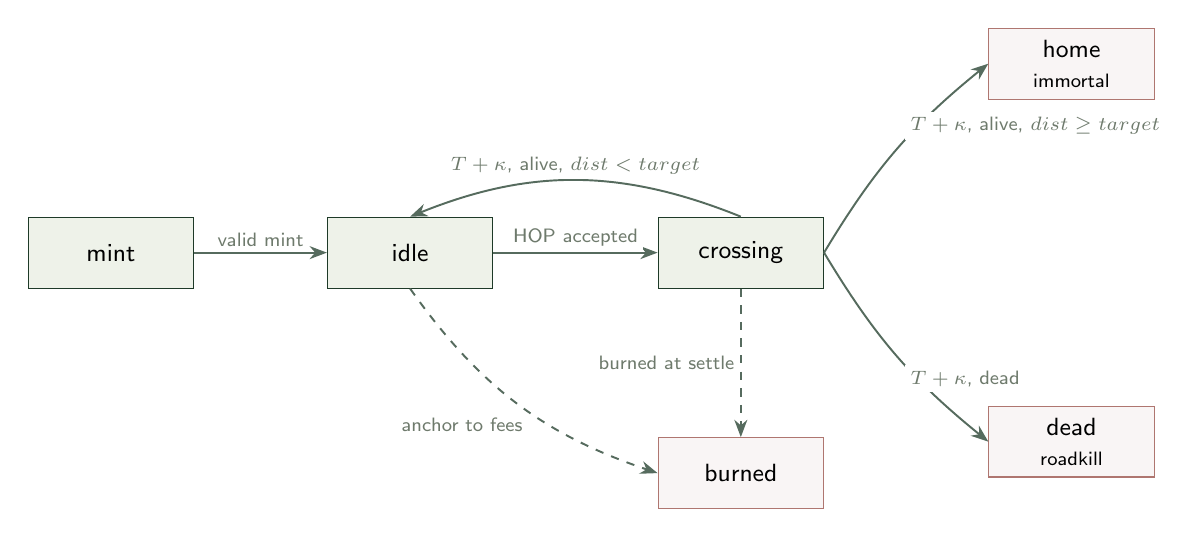
\begin{tikzpicture}[
  state/.style={draw=deepgreen, fill=pale, rectangle, minimum width=21mm,
                minimum height=9mm, font=\sffamily\small, align=center,
                inner sep=2pt},
  terminal/.style={state, draw=deadred!70, fill=deadred!5},
  arrow/.style={-{Stealth[length=2.2mm]}, draw=deepgreen!75, line width=0.7pt},
  label/.style={font=\scriptsize\sffamily, color=muted, inner sep=2pt, fill=white}
]
\node[state] (mint) at (-3.8,0) {mint};
\node[state] (idle) at (0,0) {idle};
\node[state] (crossing) at (4.2,0) {crossing};
\node[terminal] (home) at (8.4,2.4) {home\\\scriptsize immortal};
\node[terminal] (dead) at (8.4,-2.4) {dead\\\scriptsize roadkill};
\node[terminal] (burned) at (4.2,-2.8) {burned};

\draw[arrow] (mint) -- node[label, above] {valid mint} (idle);
\draw[arrow] (idle) -- node[label, above] {HOP accepted} (crossing);
\draw[arrow, dashed] (idle.south) to[bend right=18]
  node[label, below left, pos=0.55] {anchor to fees} (burned.west);
\draw[arrow] (crossing.north) to[bend right=22]
  node[label, above, pos=0.5] {$T+\kappa$, alive, $dist<target$} (idle.north);
\draw[arrow] (crossing.east) to[bend left=10]
  node[label, above right, pos=0.55] {$T+\kappa$, alive, $dist\ge target$} (home.west);
\draw[arrow] (crossing.east) to[bend right=10]
  node[label, below right, pos=0.55] {$T+\kappa$, dead} (dead.west);
\draw[arrow, dashed] (crossing.south) -- node[label, left] {burned at settle} (burned.north);
\end{tikzpicture}
\caption{The v8 frog lifecycle. \code{home}, \code{dead}, and \code{burned}
are absorbing. The dashed transitions are terminal or exceptional: an idle
frog whose anchor sat is paid to fees is burned immediately, while an
in-flight frog that is burned settles as burned at finality.}
\label{fig:lifecycle}
\end{figure}

\subsection{Transfer and burn}

A spend of the frog's outpoint without a valid crossing envelope is a
transfer: the indexer updates \code{location} and leaves the state unchanged.
No inscription is published, and no state changes. This is the simplest way
to move a frog, and it is why a transfer is invisible to the fold.

A spend that sends the anchor sat to fees marks \code{location = burned} and
sets \code{burn_height} and \code{burn_txid}. An idle frog becomes
\code{burned} immediately, because nothing else will observe the sat again.
An in-flight crossing keeps its timer and settles as \code{burned} at
finality. A wallet should not build, offer, or expose \textsc{burn} as a
feature or operation; the indexer still classifies such a spend if it is
built elsewhere.

The asymmetry is intentional. A transfer of an idle frog is a normal custody
move. A burn is irreversible, and the record must say so at the moment the
sat leaves the tracked set. For an in-flight frog, the outcome at $T+1$ has
already been frozen; destroying the sat does not undo the crossing, it only
changes how the settlement is labelled.

\subsection{Events}

The indexer publishes a re-derivable log. Each entry is keyed by
$(\mathit{block\_hash},\mathit{height},\mathit{txid},\mathit{action})$ and has
one of four shapes.

\begin{table}[H]
\centering
\small
\caption{Event payloads.}
\label{tab:events}
\begin{tabularx}{\linewidth}{@{}p{0.16\linewidth}X@{}}
\toprule
\textbf{Action} & \textbf{Payload} \\
\midrule
\code{mint} & \code{{frogger_sat, seed, name, gen}} \\
\code{transfer} & \code{{frogger_sat}} \\
\code{settle} & \code{{frogger_sat, outcome: dead|crossed, dir, wrap}} \\
\code{burn} & \code{{frogger_sat}} \\
\bottomrule
\end{tabularx}
\end{table}

The log is not a second consensus. It is a projection of the same events the
state machine applied, and it can be regenerated from the chain.
\code{outcome: crossed} means the Hopper survived that hop, not that it
reached \code{HOME}. \code{HOME} is the frog record's
\code{state = home} with \code{immortal_height = T}; the road log reads the
frog record, not the bare event. The \code{burn} action remains an
indexer/API state, not a wallet feature.

\subsection{Reorganizations}

The indexer keeps a retained window of block headers and undo journals. A
rollback replays the chain to the fork point. Timers are pure functions of
height and hash, so a reorg that replaces $T+1$ freezes a new outcome, and a
reorg that removes $T$ reopens the frog as \code{idle} and restores its card.
No manual repair is required.

\begin{invariant}{Settlement is monotone before finality}
Before $T+\kappa$, the only committed fact is the crossing itself. The
outcome hash, the wrap and the provisional verdict may be replaced by a
reorg. At $T+\kappa$, the retained window is what allows the indexer to
replay a fork without losing the ability to settle.
\end{invariant}

\subsection{A crossing in six acts}

The whole protocol can be read as six steps.

\begin{enumerate}[leftmargin=1.7em,itemsep=0.22em]
  \item The wallet derives the state output for
        $(\mathrm{sat},\mathit{mint\_id},\mathit{owner})$.
  \item The player chooses left, straight or right. The wallet signs the
        matching cross leaf with the owner key and includes funding and
        change as needed.
  \item It broadcasts one transaction. The transaction carries exactly one
        inscription, in input 0, and sends the anchor sat to output 0 at
        offset 0.
  \item The indexer admits the crossing at height $T$, freezes $r(T)$,
        records the chosen direction, and emits a \code{crossing} state. The
        art fold reports \textsc{crossing}.
  \item At $T+1$ the outcome hash is recorded and the block's wrap is
        computed. No settlement happens yet.
  \item At $T+\kappa$ the timers run: \code{home} if the distance reached the
        target, \code{idle} if the frog survived but has more to go, or
        \code{dead} if its chosen direction equals the block's wrap.
\end{enumerate}

\section{Custody: the Taproot tree that plays the game}\label{sec:custody}

\subsection{The state output}

A frog in custody is a Taproot output with the fixed internal key
\code{NUMS_XONLY}:
\begin{center}
\footnotesize\code{50929b74c1a04954b78b4b6035e97a5e078a5a0f28ec96d547bfee9ace803ac0}.
\end{center}
No discrete log of this point is known, so there is no key-path spend. The
output can only be spent through one of four leaves. The tree is balanced at
depth two: three crossing leaves $L,S,R$ (left, straight, right) and one send
leaf $X$ (transfer).

\begin{align}
h_L&=\mathrm{leaf\_hash}(L), & h_S&=\mathrm{leaf\_hash}(S),\notag\\
h_R&=\mathrm{leaf\_hash}(R), & h_X&=\mathrm{leaf\_hash}(X),\notag\\
h_{LS}&=\mathrm{branch}(h_L,h_S), & h_{RX}&=\mathrm{branch}(h_R,h_X),\notag\\
\mathit{root}&=\mathrm{branch}(h_{LS},h_{RX}), & Q&=\mathrm{taproot\_output\_key}(\text{NUMS},\mathit{root}),\notag
\end{align}
where
\begin{equation}
\mathrm{branch}(a,b)=\mathrm{tagged\_hash}(\text{``TapBranch''},
  \min(a,b)\,\|\,\max(a,b)),
\end{equation}
and
\begin{equation}
\mathrm{leaf\_hash}(s)=\mathrm{tagged\_hash}(\text{``TapLeaf''},
  \text{\code{0xc0}}\,\|\,\mathrm{compact\_size}(|s|)\,\|\,s).
\end{equation}

\begin{figure}[htbp]
\centering
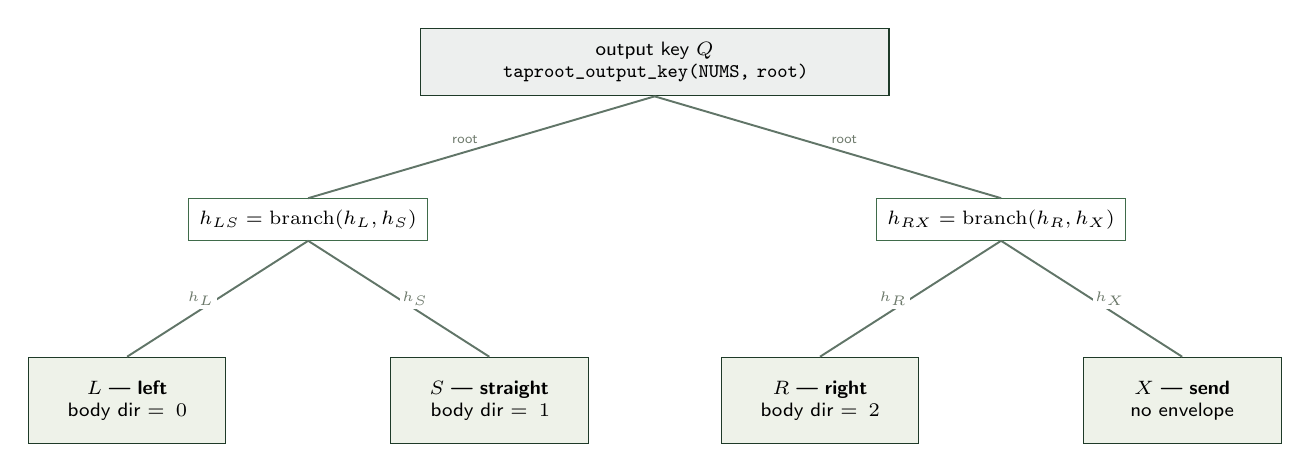
\begin{tikzpicture}[
  font=\small,
  leaf/.style={draw=deepgreen, fill=pale, rectangle, align=center,
               text width=23mm, minimum height=11mm, inner sep=3pt,
               font=\scriptsize\sffamily},
  branch/.style={draw=midgreen, fill=white, rectangle, align=center,
                 inner sep=4pt, font=\scriptsize\sffamily},
  root/.style={draw=deepgreen, fill=deepgreen!8, rectangle, align=center,
               inner sep=5pt, font=\scriptsize\sffamily, text width=56mm},
  edge/.style={draw=deepgreen!70, line width=0.7pt},
  lbl/.style={font=\tiny\sffamily, color=muted, fill=white, inner sep=1pt}
]
\node[root] (root) at (0,3)
  {output key $Q$\\\code{taproot_output_key(NUMS, root)}};
\node[branch] (ls) at (-4.4,1) {$h_{LS}=\mathrm{branch}(h_L,h_S)$};
\node[branch] (rx) at (4.4,1) {$h_{RX}=\mathrm{branch}(h_R,h_X)$};
\node[leaf] (L) at (-6.7,-1.3) {\textbf{$L$ — left}\\body dir $=0$};
\node[leaf] (S) at (-2.1,-1.3) {\textbf{$S$ — straight}\\body dir $=1$};
\node[leaf] (R) at (2.1,-1.3) {\textbf{$R$ — right}\\body dir $=2$};
\node[leaf] (X) at (6.7,-1.3) {\textbf{$X$ — send}\\no envelope};
\draw[edge] (root.south) -- node[lbl, midway, above left] {root} (ls.north);
\draw[edge] (root.south) -- node[lbl, midway, above right] {root} (rx.north);
\draw[edge] (ls.south) -- node[lbl, midway, left] {$h_L$} (L.north);
\draw[edge] (ls.south) -- node[lbl, midway, right] {$h_S$} (S.north);
\draw[edge] (rx.south) -- node[lbl, midway, left] {$h_R$} (R.north);
\draw[edge] (rx.south) -- node[lbl, midway, right] {$h_X$} (X.north);
\end{tikzpicture}
\caption{The four-leaf state output. The internal key is a nothing-up-my-sleeve
point; all leaves sit at depth two. $L$, $S$ and $R$ are the crossing leaves,
identical except for the direction byte in the body they push. $X$ is the
send leaf. There is no key-path spend.}
\label{fig:taproot}
\end{figure}

Every control block is 97 bytes:
\begin{equation}\label{eq:control}
\begin{aligned}
&[\mathit{parity}\mid\text{\code{0xc0}}]\;\|\;\text{\code{NUMS_XONLY}}\\
&\qquad\|\;\langle\text{sibling leaf hash}\rangle\;\|\;
\langle\text{sibling subtree hash}\rangle.
\end{aligned}
\end{equation}

\begin{table}[H]
\centering
\small
\caption{Control-block siblings by spent leaf.}
\label{tab:control}
\begin{tabular}{@{}lcc@{}}
\toprule
\textbf{Spent leaf} & \textbf{First sibling} & \textbf{Second sibling} \\
\midrule
$L$ (left)     & $h_S$ & $h_{RX}$ \\
$S$ (straight) & $h_L$ & $h_{RX}$ \\
$R$ (right)    & $h_X$ & $h_{LS}$ \\
$X$ (send)     & $h_R$ & $h_{LS}$ \\
\bottomrule
\end{tabular}
\end{table}

The three crossing leaves differ only in the direction byte of the body they
push (Section~\ref{sec:inscriptions}). Each leaf hash is therefore fixed when
the state output is created. Choosing a direction selects a leaf; it cannot
change the leaf's bytes. The current tree uses the
\code{FRG8CROSS}/\code{0x08} body. A state output whose sat equals
\code{GRANDFATHERED_SAT} may use the released
\code{FRG7CROSS}/\code{0x07} body and its own leaf hashes; the two versions
are never mixed in one tree.

\code{owner_xonly} is the 32-byte witness program of a BIP86 P2TR address
derived at
\begin{equation}
m/84'/\mathit{coin}'/0'/2/0,
\end{equation}
the ordinals branch. Its BIP86 even-$Y$ normalized output is the wallet's
current frog receive address and the state-leaf owner. The released
implementation tweaked the raw point without normalizing; a recovery scan
also watches that legacy address and derives the legacy state scripts. The
sender parses the recipient's P2TR address to obtain the key; a non-P2TR
destination is refused for custody.

\subsection{The cross leaf}

All three crossing leaves are the same script; only the last byte of the
pushed body (the direction) differs:
\begin{lstlisting}[language={},caption={Cross leaf template.},label={lst:cross-leaf}]
20 <owner:32>          ; PUSH32 owner
ad                     ; OP_CHECKSIGVERIFY
00                     ; OP_FALSE
63                     ; OP_IF
03 "ord"               ; PUSH 3 "ord"
01 01                  ; push tag 1
18 <content-type:24>   ; PUSH 24 "application/octet-stream"
01 03                  ; push tag 3
20 <parent:32>         ; PUSH32 mint txid (index 0)
00                     ; empty body tag
37 <body:55>           ; PUSH 55 bytes, last byte = dir; FRG8CROSS/0x08
68                     ; OP_ENDIF
51                     ; OP_TRUE
\end{lstlisting}

The first part is an ordinary \code{CHECKSIGVERIFY} against the owner key.
The second part is an ord envelope that is never executed as a condition:
\code{OP_FALSE} skips the \code{OP_IF} branch, so the envelope is data, not
control flow. The final \code{OP_TRUE} leaves a true stack value after the
signature check.

Every push is minimal. The content type is the 24-byte string
\code{application/octet-stream}, pushed with \code{0x18}. The parent tag is
the 32-byte mint txid for index $0$ --- the only reachable case, since a valid
mint carries exactly one envelope and it sits on input 0 --- or the txid plus
the minimal little-endian index (a push of length 33 to 36 bytes, opcode
\code{0x21} to \code{0x24}). The script is therefore \textbf{161 bytes} at index $0$, and up
to 165 bytes for a manually built nonzero index. The three direction leaves
are the same length; only the body's last byte differs.

The send leaf is deliberately smaller:
\begin{lstlisting}[language={},caption={Send leaf.},label={lst:send-leaf}]
20 <owner:32> ac
\end{lstlisting}
It is 34 bytes and contains no envelope. A transfer is therefore silent: it
moves the sat but publishes no state.

\subsection{Control blocks and witnesses}

A custody spend has three witness elements:

\begin{table}[H]
\centering
\small
\caption{Witness stacks for the two custody spends.}
\label{tab:witnesses}
\begin{tabularx}{\linewidth}{@{}p{0.16\linewidth}p{0.35\linewidth}X@{}}
\toprule
\textbf{Spend} & \textbf{\code{witness[0]}} & \textbf{\code{witness[1]}} / \textbf{\code{witness[2]}} \\
\midrule
hop & 64-byte BIP-340 \cite{bip340} signature $\|$ \code{0x01} (SIGHASH\_ALL) &
the chosen \code{dir} leaf script / 97-byte control block \\
transfer & 64-byte signature $\|$ \code{0x01} &
send leaf script / 97-byte control block \\
\bottomrule
\end{tabularx}
\end{table}

SPEC.md specifies that the signature is produced with the tweaked owner key
over the BIP-342 tapscript sighash of the leaf and the transaction's whole
prevouts and outputs. The reference implementation expresses that key as
\code{internal_key.tap_tweak(None)}. The SIGHASH\_ALL byte commits every
input and output, so a signature cannot be redirected to a different
transaction.

\subsection{The two-phase mint}

Ord needs an input to engrave an inscription, so a mint is a commit/reveal
pair. The commit output is a Taproot output with the BIP86 owner key
(\code{owner_xonly}) as internal key and one leaf:
\begin{lstlisting}[language={},caption={Commit output leaf.},label={lst:commit-leaf}]
<owner:32> OP_CHECKSIG OP_FALSE OP_IF <mint inscription envelope> OP_ENDIF
\end{lstlisting}
Its address is
$\mathrm{p2tr}(\mathit{owner},\mathrm{merkle\_root}(\mathrm{leaf}))$, and its
value is
\begin{equation}
1{,}000 + \mathrm{reveal\_fee\_budget}(\mathit{feerates}).
\end{equation}
The leaf demands the owner's signature. SIGHASH\_DEFAULT commits every
prevout and every output, so a copied witness cannot redirect the frog. A
legacy keyless commit, using \code{NUMS} as internal key with
\code{OP_TRUE || envelope}, remains revealable forever, but no new commit
may use it.

The reveal transaction then has the shape in Table~\ref{tab:reveal}.

\begin{table}[htbp]
\centering
\small
\caption{The mint reveal transaction.}
\label{tab:reveal}
\begin{tabularx}{\linewidth}{@{}p{0.12\linewidth}p{0.22\linewidth}X@{}}
\toprule
\textbf{Position} & \textbf{Role} & \textbf{Content} \\
\midrule
input 0 & commit spend & script path \code{[sig, leaf, control block]} \\
output 0 & frog & 1{,}000 sats to the wallet's frog P2TR key-path address \\
output 1 & mint message & OP\_RETURN \code{FRG 0x08 0x01 seed name} (\code{0x07} only for the grandfather) \\
output 2 & change & \code{m/84'/coin'/0'/1/index}, optional if $\ge$ dust \\
\bottomrule
\end{tabularx}
\end{table}

Every input uses sequence \code{0xFFFFFFFF}, so the transaction is not
replaceable. The anchor sat is the first sat of the commit output, which is
the first sat of the first funding input. Because the commit leaf embeds the
anchor sat, the commit address is derived after a probe coin-selection pass.

\subsection{Action transactions}

After the mint, a frog moves through the transactions in
Table~\ref{tab:actions}. All of them use version 2, lock time zero, and
sequence \code{0xFFFFFFFF} on every input. They are intentionally not
replaceable: a mint, prepare, hop or transfer may move an inscription or a
state card, and shaving an output to raise a fee can burn the anchor sat.

\begin{table}[htbp]
\centering
\small
\caption{The custody actions.}
\label{tab:actions}
\begin{tabularx}{\linewidth}{@{}p{0.12\linewidth}p{0.30\linewidth}X@{}}
\toprule
\textbf{Action} & \textbf{Input 0} & \textbf{Outputs} \\
\midrule
\textsc{prepare} & the frog output, P2TR key path with the tweaked frog key &
output 0 is the state output for $(\mathrm{sat},\mathit{mint},\mathit{owner})$;
outputs 1.. are funding change \\
\textsc{hop} & the state output, the leaf for the chosen direction &
output 0 is the next state output (same owner or a new P2TR owner);
outputs 1.. are funding change \\
\textsc{transfer} & the state output via the send leaf, or the mint output via
key path & output 0 is the recipient's ordinary address (any script, P2WPKH
included) \\
\bottomrule
\end{tabularx}
\end{table}

\begin{invariant}{One crossing per transaction}
A hop publishes exactly one inscription, in input 0. The anchor sat must
land in output 0 at offset 0. No funding input may carry a frog, and no
\code{FRG} envelope may appear anywhere in the crossing.
\end{invariant}

\textsc{prepare} exists only for a frog still in its mint or frog-address
output. The state leaf commits to the mint inscription id, which is created
by the mint reveal; an output of that transaction cannot contain its own
txid. The first state output is therefore created by either the first
transfer or the one-time \textsc{prepare}. After that, each crossing spends
the previous state output and creates the next one.

The player chooses $\mathit{dir}\in\{\text{left},\text{straight},\text{right}\}$
before signing; the transaction spends the matching leaf, so the body it
inscribes carries that \code{dir}. Choosing a direction is the whole of the
choice: the leaf's bytes are fixed by the state output, and the outcome is
decided by the block, not by the player. The wallet must show the chosen
direction in the preview and must not let it change after the preview is
approved.

A transfer deliberately pays the recipient's ordinary address, not a state
output. The state script commits to the mint id, which the recipient cannot
know until it has discovered the frog. The recipient re-enters custody with
\textsc{prepare} on its next action.

\subsection{Previews and the ordinary send}

A browser \textsc{send} (including \textbf{SEND ALL}), \textsc{hop},
\textsc{transfer} or \textsc{mint} is previewed before broadcast.
\textsc{send} and \textsc{transfer} display \code{PREVIEW TRANSACTION};
\textbf{SEND ALL} is titled \code{SEND ALL BITCOIN}; \textsc{mint} keeps
its \code{MINT!} button and opens the same review window; a hop is previewed
with its direction spelled out (\code{HOP LEFT},
\code{HOP STRAIGHT} or \code{HOP RIGHT}) and the leaf it will spend. The
preview shows the destination address and amount, change address and amount
(or ``one output'' for a transfer or \textbf{SEND ALL}), chosen fee rate and
actual fee in sats. A mint shows the commit and reveal txids, both change
outputs, both fees and the total size.

\code{CANCEL} performs no broadcast, persists no action and spends nothing.
Approval re-scans and refuses the preview if any input moved, an anchor's
ordinal ranges changed, or a coin gained a Hopper, then broadcasts the exact
previewed bytes. A mint approval broadcasts the commit and then the reveal
that spends it; if the reveal is rejected after the commit was accepted, the
error names the accepted commit and no mint action is recorded. A mint never
has an RBF path. Fee recommendations come from mempool.space
\code{/api/v1/fees/precise} (\code{fastestFee}, \code{halfHourFee},
\code{economyFee}); the chosen rate remains manually editable, and values
below the 1 sat/vB wallet relay floor are raised to it.

An ordinary wallet \textsc{send} is separate from these actions. Its inputs
use sequence \code{0xFFFFFFFD} (BIP125 opt-in), and the wallet may replace an
unconfirmed send only under a narrow policy: the original is a wallet-created
plain BIP84 send; the backend returns exactly the recorded serialization;
every original input is a plain, range-known, non-Hopper BIP84 coin and the
current view still contains no Hopper at those outpoints or sats; every
original output keeps its exact script and value; the replacement appends
confirmed plain BIP84 funding and one new change output; and it pays a
strictly higher absolute fee and feerate, including BIP125's incremental
relay margin. The wallet never replaces a HOPPER action. The transaction
builder recomputes the FIFO sat ranges and refuses a replacement if a known
Hopper sat would land in its fee.

\textbf{SEND ALL.} A SEND variant sweeps the plain-BTC balance into exactly
one recipient output. It selects every eligible plain BIP84 coin: complete,
value-matched ranges, no Hopper or state output, and no protected sat;
unconfirmed coins are included only when the wallet permits them. There is no
change output, and the actual fee is deducted from the total, so the recipient
receives $\mathit{totalIn}-\mathit{actualFee}$. The build refuses when the
fee consumes the balance or leaves the recipient below the P2WPKH dust limit,
and approval repeats the same exact-bytes and input checks as SEND. The
preview is titled \code{SEND ALL BITCOIN} and states that there is one output
and no change.

\subsection{Sat assignment}

Ordinals move FIFO over inputs in order. The protocol depends on three
consequences.

\begin{enumerate}[leftmargin=1.6em,itemsep=0.22em]
  \item The anchor sat is the first sat of input 0. For a mint, that is the
        first sat of the commit output.
  \item After a spend, the anchor sat is at offset 0 of output 0 if and only
        if output 0 receives value and no earlier output claims sats first.
  \item A fee is taken from the tail of the frog's range or from funding; it
        is never taken from the anchor's position.
\end{enumerate}

The wallet and the indexer both verify these properties with ordinal range
arithmetic. A coin whose ranges cannot be attributed is not spent.

\subsection{Addresses, discovery and history}

\begin{itemize}[leftmargin=1.4em,itemsep=0.3em]
  \item The mint pays the wallet's \textbf{frog address}: the BIP86 P2TR
        output at \code{.../2/0}. It never pays a BIP-84 receive address.
        Coins at the frog address are never funding candidates.
  \item The BIP-84 receive script is \textbf{fixed at \code{.../0/0}} in
        v8. This is a deliberate simplicity and recovery tradeoff, not an
        accidental gap: the watch set is fixed, paginated to exhaustion, and
        a restored wallet reuses the same script. Address rotation and
        privacy are future wallet features, not a consensus rule. The UI
        must not claim that a receive address retires.
  \item The state output's script is per
        $(\mathrm{sat},\mathit{mint\ id},\mathit{owner})$. It matches no
        derivation path. A wallet finds it by deriving the script from the
        frog record and by watching its frog address.
  \item A frog sent by a peer arrives at the ordinary address and is
        discovered by the wallet's address scan plus the indexer or ord. It
        is imported by reading its mint inscription and replaying its history
        from the mint outpoint.
  \item History is wallet-scoped, not a raw indexer feed. It merges local
        actions, events whose Hopper sat belongs to this wallet, settled
        outputs observed on its watched scripts, internal change, and mempool
        rows. A confirmed ordinary deposit or a Hopper output is retained as
        a \code{receive} row, so it stays visible after the coin is spent.
        Change from our own transactions is retained separately as a
        \code{CHANGE} row; it is never presented as an incoming
        \code{RECEIVE}. Events for unrelated public or NPC Hoppers are
        filtered out.
  \item A \code{MINT} row does not depend only on the browser that broadcast
        it. When the owned mint output is still at its mint outpoint, the
        wallet persists a chain-derived mint row, so a restored seed shows
        the same \code{MINT} and \code{HOPPER ARRIVED} rows without a local
        action ledger. A Hopper received from a peer is not at its mint
        outpoint and does not create a \code{MINT} row.
  \item Rows for one txid share its best-known height and sort as a group.
        The feed is newest first, so inside a group the newest row is on top:
        \code{HOPPER ARRIVED} $\to$ \code{CHANGE} $\to$ \code{MINT}, and
        \code{CHANGE} $\to$ \code{SEND}. A mint's commit change is grouped
        with the reveal's \code{HOPPER ARRIVED} row by the minted sat and by
        both txids. Older actions with no stored sat recover it from the
        arrival's frog/reveal record; a missing commit is read once from
        input 0 of the reveal and persisted. A missing sat is never treated
        as sat 0. Grouping is ultimately by reveal/commit txid cluster, so it
        works even when no row stores a sat. Shortened txids and addresses
        are copy buttons: the visible text is abbreviated, but the copied
        text is the complete value.
  \item The first completed refresh after the history-ledger upgrade performs
        two one-time, versioned address-history backfills: receive addresses
        the wallet handed out, and change addresses it has used. The receive
        pass recovers deposits whose coins were spent before the receive
        ledger existed and skips outgoing action/commit txids; the change
        pass recovers spent internal change and migrates older ledgers that
        had stored it as a \code{RECEIVE}. \code{RESCAN} clears both markers
        so recovery can be forced.
\end{itemize}

\begin{invariant}{No key-path escape hatch}
A state output is a UTXO spent exactly once. The body binds the sat, the mint
and the direction, so a witness cannot be replayed against another frog. The
NUMS internal key ensures that the only ways out are the four leaves.
\end{invariant}

\section{The standalone indexer}\label{sec:indexer}

\subsection{Crate boundaries}

The Rust implementation is a three-crate workspace.

\begin{table}[htbp]
\centering
\small
\caption{Indexer crates and responsibilities.}
\label{tab:crates}
\begin{tabularx}{\linewidth}{@{}p{0.24\linewidth}X@{}}
\toprule
\textbf{Crate} & \textbf{Responsibility} \\
\midrule
\code{hopper-core} & Pure protocol: envelope, v8 and legacy body, scripts, parameters,
generations, wrap, sat math, art, PNG, fold document. Depends only on
\code{sha2} (plus optional serde). \\
\code{hopper-indexer} & Pure state machine: sat tracker, rules, timers,
events, snapshots, optional redb store. Performs no network I/O; the optional
redb store is local disk persistence. \\
\code{hopper-indexer-api} & Axum HTTP API and block ingest (ZMQ/RPC or admin
POST). Owns the network and the write lock. \\
\bottomrule
\end{tabularx}
\end{table}

The separation is not cosmetic. \code{hopper-core} can be compiled for
native and mobile targets without a Bitcoin node. \code{hopper-indexer} can
be replayed from a fixture without sockets. Only the API crate knows about
ZMQ, RPC, HTTP, or authentication.

\subsection{Ingest}

The indexer always ingests from block 0. A later start cannot name coins
created earlier; a frog whose mint predates the start would look as if it had
been sent away. This is a correctness rule, not an optimization.

There are two wires, sharing the same block decoder and the same write lock.

\begin{itemize}[leftmargin=1.4em,itemsep=0.3em]
  \item \code{POST /v1/admin/block} accepts an operator or debug JSON block.
        Outside loopback it requires the admin token.
  \item bitcoind ZMQ \code{hashblock} plus RPC is the production path. On a
        new hash, the indexer fetches blocks from its tip to that hash. On a
        reorg, it rolls back to the fork and replays.
\end{itemize}

The ingest layer converts a Bitcoin transaction into a small, witness-light
structure:
\begin{lstlisting}[language={},caption={Ingest types.},label={lst:ingest}]
Tx {
    txid,
    inputs[{ prevout, value, inscription? }],
    outputs[{ value, op_return? }]
}
Block { hash, height, txs }
\end{lstlisting}
It parses the tapscript witness at \code{witness[n-2]} with the ord envelope
decoder, extracts the control block at \code{witness[n-1]}, and records the
content type, body and tag-3 parents. The state machine never touches
witnesses.

\begin{figure}[htbp]
\centering
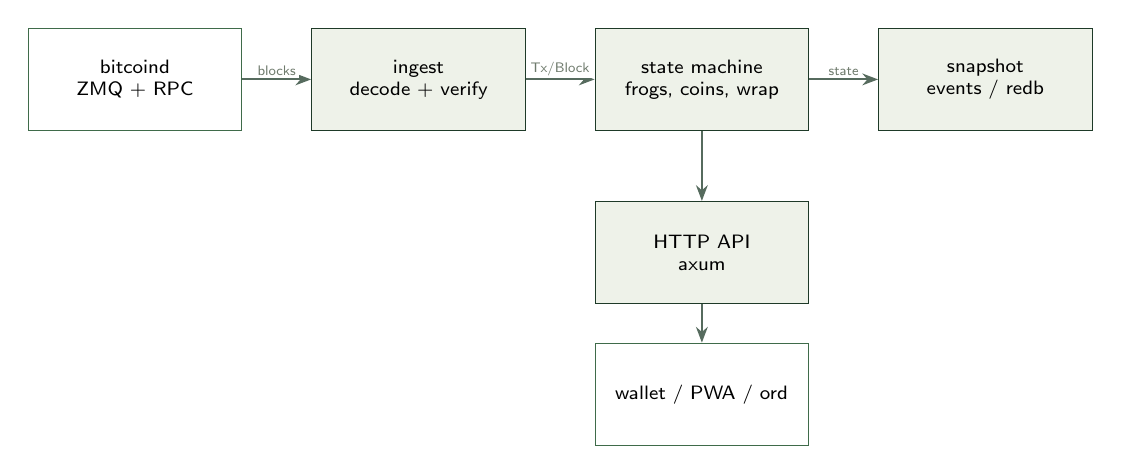
\begin{tikzpicture}[
  box/.style={draw=deepgreen, fill=pale, rectangle, align=center,
              text width=25mm, minimum height=13mm, inner sep=3pt,
              font=\scriptsize\sffamily},
  net/.style={draw=midgreen, fill=white, rectangle, align=center,
              text width=25mm, minimum height=13mm, inner sep=3pt,
              font=\scriptsize\sffamily},
  arrow/.style={-{Stealth[length=2mm]}, draw=deepgreen!75, line width=0.7pt},
  lbl/.style={font=\tiny\sffamily, color=muted, fill=white, inner sep=1pt}
]
\node[net] (node) at (0,0) {bitcoind\\ZMQ + RPC};
\node[box] (ingest) at (3.6,0) {ingest\\decode + verify};
\node[box] (engine) at (7.2,0) {state machine\\frogs, coins, wrap};
\node[box] (store) at (10.8,0) {snapshot\\events / redb};
\node[box] (api) at (7.2,-2.2) {HTTP API\\axum};
\node[net] (clients) at (7.2,-4.0) {wallet / PWA / ord};
\draw[arrow] (node) -- node[lbl, above] {blocks} (ingest);
\draw[arrow] (ingest) -- node[lbl, above] {Tx/Block} (engine);
\draw[arrow] (engine) -- node[lbl, above] {state} (store);
\draw[arrow] (engine) -- (api);
\draw[arrow] (api) -- (clients);
\end{tikzpicture}
\caption{Indexer architecture. The state machine is independent of the
network and of the HTTP layer; persistence is a projection of the same
state.}
\label{fig:indexer}
\end{figure}

\subsection{State, snapshots and the state root}

The state is a function
\begin{equation}
(\mathrm{config},\mathrm{seeds},\mathrm{chain})\;\longrightarrow\;
\mathrm{IndexState}+\mathrm{event\ log}.
\end{equation}
It contains the frog records, the coin ranges, the retained headers, the
pending timers and the tip. A canonical state root hashes the parameter
commitment, the tip (height and hash), the ordered frog records and the coin
ranges. Two indexers that agree on consensus must agree on the root; a
disagreement is a bug or a different parameter set, not a client preference.

Persistence has three layers.

\begin{itemize}[leftmargin=1.4em,itemsep=0.3em]
  \item A binary snapshot at \code{HOPPER_SNAPSHOT_PATH}, default
        \code{hopper-indexer.snapshot.bin}. The snapshot embeds the parameter
        hash; a mismatch on load is a hard error, never a migration.
  \item Append-only event segments next to the snapshot.
  \item An optional redb durable store (feature \code{redb}, path
        \code{HOPPER_DB}) holding the full state and the undo journals.
\end{itemize}

The snapshot interval defaults to 10 blocks, the retained block window to
288 blocks, and the event segment size to 4096 events.

\subsection{HTTP API}

The public surface is read-only. Administrative routes are separate and
require a Bearer token when \code{HOPPER_ADMIN_TOKEN} is set; the server
refuses a non-loopback bind without one. They are never exposed by the PWA.

\begin{table}[H]
\centering
\small
\caption{Indexer HTTP API.}
\label{tab:api}
\begin{tabularx}{\linewidth}{@{}p{0.39\linewidth}X@{}}
\toprule
\textbf{Route} & \textbf{Purpose} \\
\midrule
\code{GET /v1/status} & Tip, height, active crossings, wire version \\
\code{GET /v1/params} & Full parameter block, \code{params_hash}, chain id \\
\code{GET /v1/generation/{height}} & Generation index, start, end,
\code{required(h)} \\
\code{GET /v1/wrap/{height}} & The block's wrap ($0|1|2$); 404 until
ingested \\
\code{GET /v1/froggers} & Paginated list; \code{limit}, \code{offset},
\code{after_sat}, \code{to_sat} \\
\code{GET /v1/frogger/{sat}} & One frog record, with \code{gen},
\code{in_flight.dir} and \code{outcome.wrap} \\
\code{GET /v1/road} & In-flight crossings: $T$, direction, target, wrap,
settle height \\
\code{GET /v1/leaderboard} & Ranked by generation, then \code{dist};
\code{limit} \\
\code{GET /v1/state/root} & Canonical state root \\
\code{GET /v1/events} & Event log; \code{limit} \\
\code{GET /v1/events/stream} & Server-sent event stream \\
\code{GET /v1/mempool} & Mempool preview; needs RPC \\
\code{GET /v1/fees} & bitcoind fee estimate; never invented \\
\code{GET /v1/utxo/{txid}/{vout}} & Value, ordinal ranges, frogs,
\code{exact} flag \\
\code{GET /healthz}, \code{/readyz}, \code{/metrics} & Liveness, readiness,
metrics \\
\code{POST /v1/admin/block} & Ingest an operator/debug block \\
\code{POST /v1/admin/seed} & Bootstrap explicit ordinal ranges \\
\code{POST /v1/admin/rollback} & Roll back to a fork point \\
\bottomrule
\end{tabularx}
\end{table}

CORS is a browser read policy configured by \code{HOPPER_CORS_ORIGINS}. It
is not access control and must not be treated as one. The API never publishes
a wrap for a height it has not ingested: the outcome of a future block is not
predictable from the indexer either.

\subsection{Configuration}

\begin{table}[H]
\centering
\small
\caption{Indexer configuration. Legacy \code{FROGGER_*} names are accepted
as fallbacks.}
\label{tab:config}
\begin{tabularx}{\linewidth}{@{}p{0.43\linewidth}X@{}}
\toprule
\textbf{Variable} & \textbf{Meaning / default} \\
\midrule
\code{HOPPER_API_ADDR} & Bind address; default \code{127.0.0.1:9770} \\
\code{HOPPER_ACTIVATION_HEIGHT} & Frozen inscription cutover; default and
required \code{974,034} \\
\code{HOPPER_INSCRIPTION_ACTIVATION_HEIGHT} & Frozen cutover; default and
required \code{974,034} \\
\code{HOPPER_RATE_LIMIT_PER_MIN} & Public-read budget per caller; default
300, \code{0} disables \\
\code{HOPPER_CORS_ORIGINS} & Browser read origins; default \code{*}; not
access control \\
\code{HOPPER_SNAPSHOT_PATH} & Snapshot file; default
\code{hopper-indexer.snapshot.bin} \\
\code{HOPPER_SNAPSHOT_EVERY} & Snapshot interval; default 10 blocks \\
\code{HOPPER_RETAIN_BLOCKS} & Reorg window; default 288 \\
\code{HOPPER_EVENT_SEGMENT} & Events per append-only segment; default 4096 \\
\code{HOPPER_EVENT_RETAIN_SEGMENTS} & Old segments retained; default 0 (keep
all) \\
\code{HOPPER_SEEDS_FILE} & Bootstrap seed JSON for fresh starts \\
\code{HOPPER_INGEST_START_HEIGHT} & Must be 0 or unset; later starts are
refused \\
\code{HOPPER_ORD_URL} & Optional ord base for lazy range seeding \\
\code{HOPPER_ZMQ_ADDR} & bitcoind \code{zmqpubhashblock}, e.g.
\code{tcp://127.0.0.1:28332} \\
\code{HOPPER_RPC_URL} & bitcoind RPC; default
\code{http://127.0.0.1:18443} \\
\code{HOPPER_RPC_COOKIE}\newline \code{HOPPER_RPC_USER}\newline \code{HOPPER_RPC_PASS} & RPC authentication \\
\code{HOPPER_NETWORK} / \code{HOPPER_GENESIS_HASH} & Published chain
identity \\
\code{HOPPER_ADMIN_TOKEN} & Bearer token for \code{/v1/admin/*}; a
non-loopback bind without it is refused \\
\code{HOPPER_DB} & Optional redb path \\
\code{HOPPER_DB_CACHE_MIB} & redb page cache in MiB; 0/unset uses redb's
default \\
\code{HOPPER_ENGINE=store} & Keep only a block-sized overlay in memory \\
\code{HOPPER_REINDEX=1} & Discard the durable store \\
\bottomrule
\end{tabularx}
\end{table}

The legacy \code{FROGGER_*} spellings are read as fallbacks so an existing
deployment can migrate without editing its service file.

\subsection{Seeding}

Ordinal ranges ultimately come from the chain. A fresh indexer ingests from
genesis, but a deployment that starts from a snapshot, or that is handed a
UTXO it never saw move, can be given explicit ranges:
\begin{center}
\begin{minipage}{0.88\linewidth}
\begin{lstlisting}[language={},caption={Admin seed request.},label={lst:seed}]
POST /v1/admin/seed
{
  "utxos": [
    { "txid": "<display hex>", "vout": 0,
      "ranges": [[start, end]] }
  ]
}
\end{lstlisting}
\end{minipage}
\end{center}
A coin whose ranges were never observed is a shadow sat. A mint on one is
rejected as \texttt{MintAnchor\allowbreak Untracked}. Seeding is an operator bring-up step,
not a consensus rule.

\subsection{Rejections}

No malformed input is chain-invalidating. A rejection leaves state unchanged
while sat movement still applies. The closed set lives in
\code{hopper-indexer/src/types.rs} as \code{RejectionReason}; its families
are:
\begin{itemize}[leftmargin=1.4em,itemsep=0.2em]
  \item mint anchor issues (untracked, shadow, already carrying a frog);
  \item inscription content type and mint-body digest issues;
  \item crossing body, parent, leaf or control-block issues;
  \item the direction set: \code{dir > 2}, the spent leaf is not the
        \code{dir} leaf, or the control block is not the matching row of
        Table~\ref{tab:control};
  \item crossing outpoint and output-position issues;
  \item crossing on a non-idle frog;
  \item funding inputs carrying a frog;
  \item mixed \code{FRG} envelope;
  \item parameter-hash mismatch.
\end{itemize}

A rejected transaction is not a reorg and not a chain failure. It is a
protocol message that the state machine declined to apply. The API also
refuses to serve a mismatched parameter set: \code{GET /v1/params} publishes
the hash, wire version and chain identity, and the wallet refuses to sign
without a matching \code{network}. Missing identity is not permission.

\begin{invariant}{Deterministic replay}
Given the same blocks, the same seeds and the same parameter set, the
indexer produces the same state root and the same event log. Network
topology, arrival order and wall-clock time are not inputs.
\end{invariant}

\section{The wallet and the PWA}\label{sec:wallet}

\subsection{Keys and the vault}

A wallet is a 12-word BIP-39 mnemonic. The full 64-byte BIP-39 seed is
derived through BIP-32 to
\begin{equation}
m/84'/\mathit{coin}'/0',
\end{equation}
with coin type 0 on mainnet and 1 elsewhere. The receive script is fixed at
$m/84'/\mathit{coin}'/0'/0/0$ and change addresses are
$m/84'/\mathit{coin}'/0'/1/i$; both are P2WPKH. The fixed receive script is a
deliberate v8 simplicity and recovery tradeoff. The watch set is fixed,
paginated to exhaustion, and a restored wallet reuses the same script;
address rotation is a future feature, not a consensus rule.

The ordinals branch is different. The branch is derived at
\begin{equation}
m/84'/\mathit{coin}'/0'/2/0.
\end{equation}
The branch point is normalized to even $Y$ and tweaked once with an empty
merkle root (the BIP86 \cite{bip86} tweak). The resulting output key is the
32-byte \code{owner}: it is the owner in the mint commit leaf and the commit
output's internal key, the owner committed by the four state leaves, the key
that signs crossings and transfers, and the wallet's current frog receive
address. The untweaked branch key is not itself an owner. The released
implementation tweaked the raw point without normalizing; a recovery scan
also watches that legacy address and derives the legacy state scripts.
Migration is explicit: a \code{migrateLegacyFrog} transfer moves the sat to
the current address. The old path is never rewritten in place. This key is
not used for funding. Coins at the frog address are never candidates for coin
selection, because spending one as fee would burn a frog.

The vault stores the BIP-39 entropy sealed with AES-256-GCM under a
non-extractable WebCrypto key-encryption key held in IndexedDB. Creation
writes, reads back and verifies the ciphertext before reporting success; a
storage denial is an error, never a ``sealed'' vault. The public ledger
(addresses, UTXOs, frog records, history) is stored separately. The ledger is
re-derivable from the chain; the 12 words are the only backup.

\begin{table}[htbp]
\centering
\small
\caption{Wallet derivation paths.}
\label{tab:derivation}
\begin{tabularx}{\linewidth}{@{}p{0.36\linewidth}p{0.16\linewidth}X@{}}
\toprule
\textbf{Path} & \textbf{Script} & \textbf{Purpose} \\
\midrule
$m/84'/\mathit{coin}'/0'/0/0$ & P2WPKH & Receive (fixed in v8) \\
$m/84'/\mathit{coin}'/0'/1/i$ & P2WPKH & Change \\
$m/84'/\mathit{coin}'/0'/2/0$ & P2TR & Frog receive and state owner \\
\bottomrule
\end{tabularx}
\end{table}

\subsection{Chain access}

The wallet has two HTTP ports, chosen by URL.

\paragraph{Esplora.} For an \code{https://} endpoint, the wallet uses the Esplora API \cite{esplora}:
\code{/blocks/tip/height}, \code{/address/{a}/utxo},
\code{/address/{a}/txs}, \code{/address/{a}/txs/chain[/{after_txid}]},
\code{/tx/{txid}/hex}, \code{/blocks/tip/hash},
\code{/block-height/{h}}, \code{/fee-estimates}, and \code{POST /tx}.
Address history is paginated to exhaustion; the first 50 rows are never
treated as complete.

\paragraph{Electrum over WebSocket.} For a \code{ws://} or \code{wss://}
endpoint, the wallet speaks JSON-RPC 2.0 and uses
\code{blockchain.scripthash.*}, \code{blockchain.transaction.get},
\code{blockchain.block.header(s)}, \code{blockchain.estimatefee}, and
\code{blockchain.transaction.broadcast}. A relay (\code{frogger-relay}) can
bridge raw TCP.

Discovery comes from the HOPPER indexer
(\code{/v1/froggers}, \code{/v1/frogger/{sat}}, \code{/v1/utxo/...}) or,
without an indexer, from stock ord (\code{/r/utxo/...},
\code{/content/{id}}, \code{/r/blockheight}). Ranges are mandatory before a
coin may be spent. An unattributable coin still counts in the balance, but it
is displayed as unspendable rather than spent blindly.

\paragraph{Tip catch-up.} Address scans are gated on the tip
$(\mathit{height},\mathit{hash})$: outside the catch-up window below, an
unchanged tip with no wallet transaction in flight costs no address queries.
The tip endpoint can publish a block before the address index has that
block's transactions. After an automatic pass that observes a new tip, the
wallet must therefore run two further full passes at
\code{TIP_RECHECK_MS} (about 1.2 s) even though the tip is unchanged. Those
passes bypass the gate and read the addresses again; only then may the gate
skip them. Without this grace window, the first pass could record the new tip
while holding the old UTXO set and the gate would keep the stale view until
the next block or a forced \code{RESCAN}. A manual \code{RESCAN} is a forced
pass; it does not itself create this automatic grace window.

\paragraph{Scan repaint.} A completed scan is also a UI repaint event. If it
lands while a foreground action holds the busy overlay, the repaint must be
queued and applied when that action releases the UI, not dropped. Otherwise
the Road or Pond can stay on the previous snapshot until the next block or a
manual \code{RESCAN} even though the wallet state is current.

A mint reveal is also self-describing: its tapscript witness contains the
canonical v8 body (or the v7 body for the grandfather), and output 0 pays the
wallet's ordinals address. A wallet
may recover an idle mint record from that witness when neither an indexer
nor ord answers, verifying the seed, sat and full body before trusting it.
This recovers mints paid directly to the wallet's ordinals address. It does
not recover a frog transferred in later, whose new output carries no mint
body; that discovery requires the indexer, or a working ord range view and a
record source.

\subsection{Screens and interaction}

The interface is a single-page PWA with the following screens:

\begin{center}
\small
\begin{tabular}{@{}llll@{}}
\toprule
Wallet & History & The Pond & The Road \\
Mint & Leaderboard & Detail & Bio \\
\bottomrule
\end{tabular}
\end{center}

\noindent
These are supplemented by onboarding (choose, show, confirm, recover,
mistake), the intro, an eight-page rules walkthrough, the $\equiv$ drawer,
send and receive sheets, the address book, backup words, a QR scanner, the
dead-frog page, and settings.

The visual language is fixed: dark lily-pad green \texttt{\#18241a}, card
\texttt{\#223226}, accent \texttt{\#f0c83c}, 8-bit monospace, square corners,
bark-framed buttons, lily-pad-bordered floating windows, and 16$\times$16
deterministic frog sprites. The art is generated from the seed, not fetched
from a server.

The road screen asks one question: \textbf{LEFT}, \textbf{STRAIGHT} or
\textbf{RIGHT}. The chosen button is the direction committed in the crossing
body and the leaf spent; the preview names it, and it cannot change after
approval. The screen states the rule in one line: the next block picks one
direction, and a Hopper that picked it dies. A frog's card shows its
generation badge (\code{G1}, \code{G2}, \ldots), its crossing count beside
the road mark, and \code{RIP} before the name once it is dead. Each settled
hop gets one road-log row. A crossed row says \textbf{survived}; it says
\textbf{came home} only when that settle's \code{immortal_height} is the
crossing height for the row ($\mathit{row.height}-\kappa$). A dead row says
\textbf{died}. If the frog record is absent, for example after a transfer
out of this wallet, the row is conservative and says \textbf{survived}
rather than claiming \code{HOME}.

\begin{figure}[htbp]
\centering
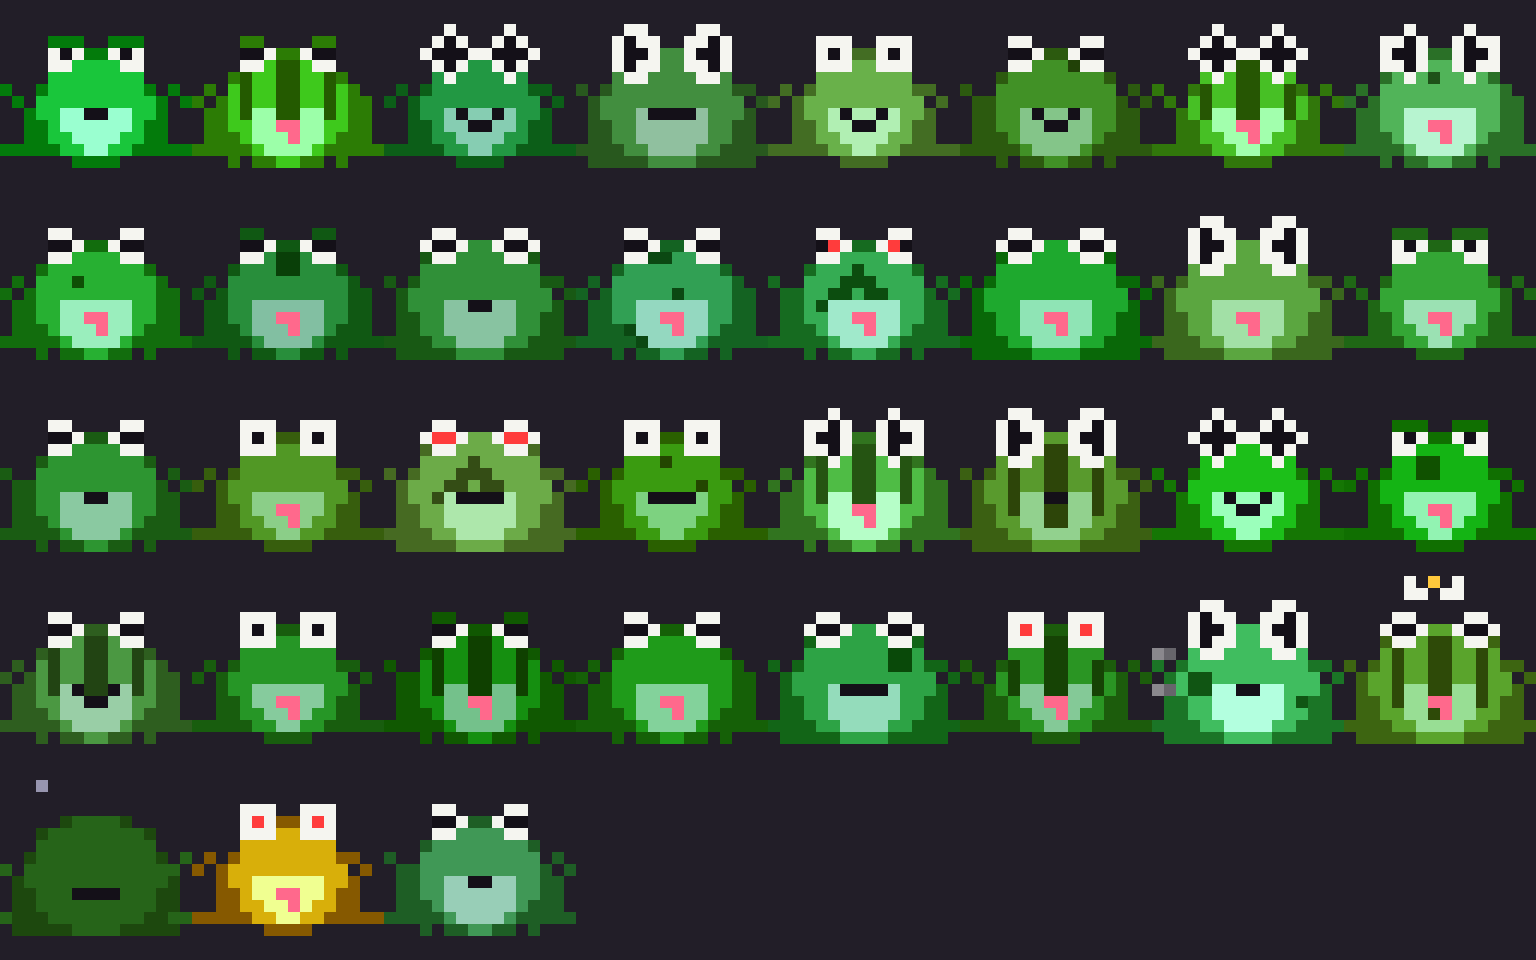
\includegraphics[width=0.82\linewidth]{figures/spritesheet.png}
\caption{Deterministic 16$\times$16 frog sprites. The same seed produces the
same sprite in the Rust implementation, the JavaScript wallet and the
inscribed fold.}
\label{fig:sprites}
\end{figure}

\subsection{Sound}

The score is one MIDI file (\code{music.mid}) played by \code{sound.js}. The
player parses the file once, maps ticks to seconds through the tempo map,
schedules notes with a 400 ms lookahead, and loops at the score's length.
Each note is one periodic-wave voice with a harmonic stack falling as
$1/k^{1.15}$, a 4 ms attack, and a pitch-dependent decay. The signal chain is
a 45 Hz highpass, a $+2.5$ dB shelf at 1.5 kHz, a compressor at $-16$ dB with
a 3.5:1 ratio, and a master gain. The gain is $0.5\cdot v^2$ for volume $v$.
Mute wins over volume, and nothing sounds before a user gesture.

\subsection{Emergency descriptor export}

The seed words are the only backup, but they do not describe how a custody
output is built. The wallet therefore offers \textbf{EXPORT EMERGENCY
DESCRIPTORS} in settings: one plain-text JSON document (also delivered as a
QR) that is enough for another taproot-capable tool to spend every staged
address without this wallet.

A \emph{staged address} is the P2TR state output of a frog. Per frog the
export carries:
\begin{center}
\begin{minipage}{0.92\linewidth}
\begin{lstlisting}[language={},caption={Per-frog emergency export fields.},label={lst:emergency}]
sat, gen, dist, state, name
mint_id            "<txid>i<index>"
state_outpoint     "<txid>:<vout>"      (when known)
state_value        sats
owner_xonly        32-byte hex
internal_key       50929b74...3ac0
output_key         32-byte x-only output key of the staged address
leaves[]           { dir, script_hex, leaf_hash, control_block }
send_leaf          { script_hex, leaf_hash, control_block }
descriptor         tr(<internal>,{raw(<L>),raw(<S>),raw(<R>),raw(<X>)})#checksum
\end{lstlisting}
\end{minipage}
\end{center}
A Hopper on a legacy path exports the released owner; a v7-wire Hopper also
uses the \code{FRG7CROSS} leaves. \code{owner_xonly} is that legacy owner.
Before displaying the document the wallet rebuilds each output key and
compares it with the scanned state scriptPubKey; a mismatch removes that frog
from the export.

and once for the wallet:
\begin{center}
\begin{minipage}{0.92\linewidth}
\begin{lstlisting}[language={},caption={Wallet-level emergency export fields.},label={lst:emergency-wallet}]
type               "hopper-v8-emergency"
version            1
network            mainnet | testnet | signet | regtest
fingerprint        BIP-32 master fingerprint (8 hex)
owner_path         m/84'/<coin>'/0'/2/0
descriptor         tr(<internal>,{raw(<L>),raw(<S>),raw(<R>),raw(<X>)})#checksum
                   (present only when exactly one staged tree; null otherwise)
generated_at       ISO-8601 UTC
tip_height         the height the export was built at
\end{lstlisting}
\end{minipage}
\end{center}

Each \code{descriptor} line uses the BIP-380 checksum and the miniscript
\code{raw()} fragment for that frog's four leaves. Many signers cannot parse
raw leaves, so the \code{leaves[]} hex and control blocks are the
authoritative form; the per-frog descriptor is a convenience for tools that
can. The wallet-level descriptor is present only when exactly one tree is
staged; with more than one it is \code{null}, and the per-frog descriptors
are the complete set.

Rules:
\begin{itemize}[leftmargin=1.4em,itemsep=0.25em]
  \item no seed words, no private keys, no xprv. The export is a \emph{layout}
        backup, not a key backup: whoever holds it still needs the seeds;
  \item the signing key is the BIP-32 key at \code{owner_path}, tweaked once
        with \code{TapTweak(P)} and an empty merkle root (the BIP86 tweak);
        the leaf's \code{owner_xonly} is the resulting output key. Spending
        uses leaf version \code{0xc0} and SIGHASH\_ALL (\code{0x01}), with the
        script and control block from \code{leaves[]};
  \item a receiving tool must verify the export before trusting it: rebuild
        each leaf hash, each branch, the root, the output key and every
        control block from the export's own bytes, and compare the result
        with the on-chain scriptPubKey of \code{state_outpoint}. The wallet
        runs the same check before it displays the export;
  \item the export is public data about the wallet's holdings. It is shown
        behind a confirmation and is never logged, uploaded, or put in a URL;
  \item the export is a snapshot, and every hop, prepare or transfer changes
        a state outpoint. The wallet stamps \code{tip_height} and regenerates
        the export after every action; a tool that sees a state outpoint
        already spent must discard the entry rather than guess.
\end{itemize}

\subsection{Wallet safety invariants}

These are mandatory before any transaction is signed or broadcast.

\begin{enumerate}[leftmargin=1.7em,itemsep=0.25em]
  \item \textbf{Complete ranges.} Every funding or state input has non-empty
        ordinal ranges whose lengths sum to its value. An empty
        ord/indexer answer is not proof that a coin has no inscription.
  \item \textbf{FIFO assignment.} The wallet recomputes the sat ranges of
        the exact signed outputs. A transfer, \textsc{prepare} or hop must
        place the Hopper sat in output 0 at offset 0; a send must not place
        any known protected sat in a recipient output, change, or the fee.
        RBF and the approval path repeat this proof.
  \item \textbf{Asset recheck.} Hop, prepare, transfer, send and mint
        revalidate every live input immediately before broadcast. The old
        exemption for send and mint is removed.
  \item \textbf{State discovery.} A state script alone never proves its sat
        ranges. Local discovery asks ord or the indexer for complete ranges
        and marks the coin unspendable until they match the value and
        contain the frog sat.
  \item \textbf{Recovery is fail-closed.} A restore paginates address
        histories to exhaustion, treats \code{more} or \code{null} as
        incomplete, reads at most a bounded checkpoint, and never
        synthesizes a range or a mint sat from a document.
  \item \textbf{Reorg identity.} Scan gates and outcome-hash caches are
        keyed by $(\mathit{height},\mathit{tip\ hash})$, not height alone.
        A same-height hash change forces a fresh pass.
  \item \textbf{Vault durability.} Vault creation writes, reads back and
        verifies the ciphertext; a storage failure is an error. Refresh
        summaries carry public keys only.
  \item \textbf{Service bounds.} Public reads are rate-limited, default
        300 per minute per caller; diagnostic \code{/v1/state/root} is not a
        hot path; and no state lock is held across an outbound ord call.
  \item \textbf{Scan freshness.} A new automatic tip gets two
        gate-bypassing catch-up passes (\code{TIP_RECHECK_MS}, about 1.2 s)
        so a lagging address index cannot freeze the UTXO view. A completed
        scan repaints the current view; if a foreground action owns the
        overlay, the repaint is queued and applied on release, never dropped.
\end{enumerate}

\subsection{The user's trust boundary}

The wallet never sends the mnemonic or the sealed entropy to a server. It
signs locally. It refuses a mint or a hop if the indexer's
\code{params_hash} differs from the embedded one, if the indexer does not
answer the parameter gate, or if its \code{network} does not match the
wallet's. It refuses a non-P2TR destination for custody. It refuses to spend
a coin whose ordinal ranges it cannot attribute. It never replaces a HOPPER
action with RBF. These refusals are part of the wallet's safety model, not UI
preferences.

\begin{invariant}{The wallet is not a custodian}
A wallet can be lost, replaced, or run offline. The frog remains a UTXO on
Bitcoin. Recovery is the 12 words; the public ledger is a cache.
\end{invariant}

\section{Security analysis}\label{sec:security}

\subsection{Threats and mitigations}

\begin{table}[H]
\centering
\small
\caption{Threats and protocol-level mitigations.}
\label{tab:threats}
\begin{tabularx}{\linewidth}{@{}p{0.29\linewidth}X@{}}
\toprule
\textbf{Threat} & \textbf{Mitigation} \\
\midrule
Forge a crossing & The chosen cross leaf requires an owner signature and a
canonical 55-byte body. The body binds the sat, mint txid, mint index and
direction; the state output is a one-time UTXO. \\
Replay a witness on another frog & The body and the parent tag both name the
mint; the state output commits to the owner. A copied witness fails
\code{CHECKSIG}, the body check, or the spent-leaf check. \\
Replay a witness with a different direction & The direction is the last byte
of the body pushed by the leaf, and the leaf hash is committed by the control
block. A witness that spent the left leaf cannot authorize a straight or
right body. \\
Counterfeit a mint & A mint requires exactly one inscription reveal in input
0, no pointer, the correct content type, the canonical v8 body digest, and a
first sat that is tracked and frog-free. The v7 digest is accepted only for
the grandfathered sat; v6 and every other v7 mint are rejected. \\
Hide a death & The fold derives the wrap from $H(T+1)$ and the direction in
the body. The static band never prints a count it cannot know. \\
Choose the outcome & The author chooses $T$ and the direction, not
$H(T+1)$. The target is frozen at $T$; the wrap does not exist when the
crossing is signed. A block producer can influence the candidate hash or
withhold a block, but that is miner influence, not player agency. \\
Blame another Hopper for a block's wrap & The wrap is global and depends only
on the block hash. One frog's death says nothing about another frog's sat or
owner. \\
Kill without publishing & A transfer publishes nothing, so a frog cannot be
killed without publishing a crossing. A burn is a separate, observable
terminal event. \\
Pointer attack & HOPPER never writes a pointer tag, and a mint carrying one
is rejected. The inscription stays on the anchor sat. \\
External-origin phishing & The mint document contains no external URL. A
viewer with different recursion semantics sees the static band, not a
third-party page. \\
Accidental burn & The wallet never uses the frog address for funding and
refuses to spend a coin whose ranges it cannot attribute. \\
Parameter confusion & The parameter hash is committed in snapshots and
checked by the wallet before mint or hop. A mismatch is a hard error. A
\code{generation_len} that does not match its formula is rejected. \\
Indexer lies & The indexer is not in the art's trust path. The viewer's own
ord node supplies the satpoints, bodies, raw transactions and block hashes
used by the fold. \\
Fabricated child & A body is not believed because it names the right parent.
The fold checks the child's sat and satpoint, then proves from the raw
transaction that input 0 spent the canonical state leaf for the body's
direction. A body pasted into a funding input, or an ordinary output-only
deposit, fails the proof and renders the fold unverified. \\
Reorg & Timers are pure functions of height and hash. The indexer replays to
the fork point; the fold simply asks again. \\
\bottomrule
\end{tabularx}
\end{table}

\subsection{Properties}

The following statements are informal but precise enough to test.

\begin{enumerate}[leftmargin=1.7em,itemsep=0.35em]
  \item \textbf{Unforgeability.} Under the security of BIP-340 signatures on
        secp256k1, an adversary without the owner key cannot produce a
        witness that passes a cross or send leaf with a valid sighash.
  \item \textbf{Direction binding.} The direction is part of the body, the
        body is pushed by the leaf, and the leaf hash is committed by the
        control block and the output key. A crossing cannot be re-labelled
        with another direction, and a witness cannot be replayed with one.
  \item \textbf{No replay across frogs.} A state body names
        $(\mathrm{sat},\mathit{mint\_txid},\mathit{mint\_index})$, and the
        state output is spent once. A witness for one frog cannot satisfy
        another frog's state output or body check.
  \item \textbf{Proof-checked public verifiability.} The fold reconstructs
        state from the mint document, the crossing inscriptions, the raw
        transactions, the tip and block hashes. A body-valid child without a
        valid canonical spend makes the fold unverified rather than
        optimistic. No secret is required and no HOPPER-specific server is
        authoritative.
  \item \textbf{Outcome independence.} The verdict depends on $H(T+1)$, which
        is not known when the crossing is signed, and on the direction the
        owner committed. The owner can time the crossing and pick a
        direction; it cannot select a favorable hash.
  \item \textbf{Deterministic replay.} The state machine is a pure function
        of blocks, seeds and parameters. Two honest indexers with the same
        inputs produce the same state root and event log.
  \item \textbf{Fail-closed art.} If the fold cannot fetch a child, verify a
        satpoint or raw proof, complete pagination, or run JavaScript, the
        document presents the static band or the unverified band with an
        unknown count. It does not claim the frog is alive, and it does not
        claim \code{HOME}.
\end{enumerate}

The first three properties are the custody argument. The fourth is
proof-checking plus the game argument. The fifth and sixth are the
infrastructure arguments. The seventh is the presentation argument.

\subsection{Limitations and honest assumptions}

\begin{warnbox}{What HOPPER does not promise}
\begin{itemize}[leftmargin=1.2em,itemsep=0.25em]
  \item \textbf{Liveness.} A transaction can be censored or fee-starved. The
        protocol decides what happens after confirmation, not when
        confirmation occurs.
  \item \textbf{Privacy.} Addresses and sat histories are public. The design
        is self-custodial, not anonymous. The global wrap also correlates
        every Hopper in a block: one block-wide coin flip, not one per frog.
  \item \textbf{Data availability.} The art, state bodies and raw
        transactions must remain retrievable from the ord node or another
        index. A viewer that cannot fetch them shows the fallback or
        unverified band.
  \item \textbf{Legacy reveals.} A keyless commit made before the signed
        commit rule remains revealable forever. No new commit may use that
        form.
  \item \textbf{Discovery.} A wallet that cannot see the chain or a trusted
        index may not find a frog sent to it. The frog still exists; the
        wallet simply has not discovered it.
  \item \textbf{Rule changes.} The rules are fixed for wire version
        \code{0x08}. A change requires a new wire version; it cannot be
        deployed by editing an indexer's configuration. The single
        grandfathered v7 Hopper is a custody exception, not a general
        compatibility mode.
  \item \textbf{Wrap bias.} The modulo is biased toward left by one part in
        $2^{32}$. This is negligible for the game and is part of the
        consensus definition.
\end{itemize}
\end{warnbox}

\subsection{Why the extra transaction is unavoidable}

A state leaf names the mint inscription id. The id contains the mint reveal
txid. An output created by the reveal transaction cannot contain that txid,
because a transaction cannot commit to its own hash. The first state output
must therefore be created by a later transaction: either the first transfer
or the one-time \textsc{prepare}. This is not an implementation artifact; it
is a consequence of self-referential identity on a hash-linked ledger.

The alternative --- omitting the mint id from the state leaf --- would make
the custody script independent of the frog's identity and would weaken
replay resistance. HOPPER chooses the extra transaction and keeps the binding.

\subsection{Compatibility notes}

Three compatibility rules are normative and easy to misread.

\begin{enumerate}[leftmargin=1.6em,itemsep=0.25em]
  \item Version 8 is the current deployment. The envelope version
        (\code{0x08}), the 55-byte body, the four-leaf tree, the proof-checked
        fold and the art all changed. A v8 indexer accepts exactly one v8
        mint-body digest. For \code{GRANDFATHERED_SAT} only, the released v7
        envelope, digest, \code{V7} body and \code{FRG7CROSS}/\code{0x07}
        state path remain valid. Every other v7 mint or crossing is rejected,
        and v6 bodies are rejected. The v7 card's embedded fold is immutable
        and predates the proof check; it is not an authoritative art oracle.
  \item The indexer accepts both minimal and PUSHDATA1 spellings of short
        pushes in an ord envelope. The reference encoder emits minimal
        pushes, and byte-exact fixtures use them, but the parser is lenient
        in the same places ord is lenient.
  \item The wrap must be computed with exactly
        \code{u32LE(H(B)_internal[0..4]) mod 3}. A wider word, a rejection
        scheme, or a hash of the hash changes the outcome and is not v8.
\end{enumerate}

These rules do not change the game. They keep old bytes valid where they
must be, and they make the decoder match the ecosystem it lives in.

\section{Validation}\label{sec:validation}

The implementation is accepted only when the obligations in
Table~\ref{tab:tests} pass. They are deliberately stated as cross-language
properties, not as unit-test counts.

\begin{table}[H]
\centering
\small
\caption{Test obligations.}
\label{tab:tests}
\begin{tabularx}{\linewidth}{@{}p{0.22\linewidth}X@{}}
\toprule
\textbf{Area} & \textbf{Obligation} \\
\midrule
Golden vectors & JavaScript and Rust produce identical \code{required}
across a generation boundary (5, 6, 25 for the whole hold, then 5 again),
the wrap \code{u32LE(H)[0..4] mod 3}, the 55-byte \code{FRG8CROSS} body,
the envelope, the parent tag, the v8 mint-body digests and the one v7
grandfather digest for pinned fixtures. \\
Wire bytes & The three 161-byte crossing leaves, the send leaf, the 97-byte
control block for each of the four leaves, the commit leaf and the witnesses
are byte-exact; parse back with the ord decoder; verify every control block
against the output key. \\
Fold parity & The embedded fold and the indexer answer the same
$(\mathrm{state},\mathrm{dist},\mathrm{gen})$ for the same crossing set,
including a block where every frog that hopped the wrap dies and every other
frog survives; a body-valid child with a missing, false or non-canonical raw
proof yields \emph{unverified}; a body pasted into a funding input or an
output-only deposit cannot count; duplicate and pre-finality crossings yield
\emph{unverified}; incomplete pagination is never a lower-bound count. \\
Consensus & Every acceptance and rejection in Section~\ref{sec:game},
the frozen activation height and the absence of a lenient mode, the
grandfathered-sat v7 path, reorgs, snapshots, the parameter hash, and a
\code{generation_len} that does not match its formula. \\
Renderers & The static card with JavaScript off shows the name and the
\code{G} badge but never a number; the proof-checked live fold shows
\nameband{ N}, \texttt{RIP }\texttt{NAME} and \texttt{HOME} against a mocked
\code{/r/} server; a missing or false raw proof shows \code{NAME}
\roadglyph{} \code{---} with no count and no \code{HOME}; no external host in
the body; the fold derives the outcome from the block hash without asking the
indexer. \\
Emergency export & Rebuild every leaf, control block and the output key from
the exported JSON alone and compare with the staged scriptPubKey; the export
contains no seed, xprv or private key; a stale \code{tip_height} is
detected. \\
App & Onboarding, keys, the fixed receive script, mint, prepare, the three
hop choices, transfer, ordinary SEND, SEND ALL (one output, no change, fee
from the swept total), history, the generation badge, display of
unattributable coins, and sound mute/volume persistence; an automatic new tip
owes two gate-bypassing catch-up passes, a scan repaint during a busy action
is applied when the action releases the UI, and the road log distinguishes
\textbf{survived} from \textbf{came home} using \code{immortal_height}. \\
\bottomrule
\end{tabularx}
\end{table}

\subsection{Reference vectors}

The following values are pinned by the reference deployment. They are
regression anchors, not additional consensus constants: the consensus
constants are the parameters in Section~\ref{sec:parameters}.

\begin{table}[H]
\centering
\small
\caption{Reference deployment vectors.}
\label{tab:vectors}
\begin{tabularx}{\linewidth}{@{}p{0.33\linewidth}X@{}}
\toprule
\textbf{Item} & \textbf{Value} \\
\midrule
$G$ & \code{974034} \\
Generation length $L$ & \code{6480} \\
$H_{\rm params}$ & \footnotesize\code{d466f8db3efa330dc92444274675804e47ec76b62393eeae88063ef764bcf72f} \\
Mint body digest\newline
seed \code{0x9058d0fa}, sat \code{1000000000000},\newline
name \code{Hopkinson}, \code{gen_hint} 1 &
\footnotesize\code{6ed060bc3186993e284e6655dcd082f4187ddde5b37051d8028a4e03cdea7ecf} \\
Mint body digest\newline
seed \code{0x00005eed}, sat \code{2099999999999},\newline
empty name, \code{gen_hint} 1 &
\footnotesize\code{1a3ba825615d0168af07cef7fc5ccf42aed819ef6e67eb868ac099fbc10b0aa5} \\
Grandfathered sat & \code{1,965,983,893,977,665} \\
v7 grandfather digest\newline
seed \code{0x9058d0fa}, sat \code{1000000000000},\newline
name \code{Hopkinson}, \code{gen_hint} 1 &
\footnotesize\code{18c566cc68856b41f4a71ac9bd0b39e57ed9ef25461798d8677ce490d1ee7dca} \\
Crossing leaf length & \code{161} bytes at mint index 0 \\
Send leaf length & \code{34} bytes \\
\bottomrule
\end{tabularx}
\end{table}

The mint digests are for the single current \code{live_v8_html}. The released
v7 digest is accepted only for the grandfathered sat, which is itself a
regression anchor. A v6 body is not an additional accepted value; it is a
different protocol.

\subsection{Conformance discipline}

Three habits keep the two implementations aligned.

\begin{enumerate}[leftmargin=1.6em,itemsep=0.25em]
  \item Constants live in one place per language, and the parameter hash is
        computed from the canonical bytes rather than hard-coded.
  \item Wire fixtures are generated once and checked into both test suites;
        no test constructs its own expected bytes from the code under test.
  \item The fold and the state machine are tested against the same synthetic
        crossing set, so a disagreement is a protocol bug rather than a UI
        bug.
\end{enumerate}

\begin{invariant}{Test the bytes, not the prose}
A specification claim that is not pinned by a byte fixture is a comment.
The wire tests are the executable form of this paper.
\end{invariant}

\section{Related work}\label{sec:related}

HOPPER sits at the intersection of ordinal theory, inscription protocols and
Taproot-based custody.

\paragraph{Ordinal theory and inscriptions.}
Ordinal theory assigns a number to every sat and defines how sats move
through transactions \cite{ordinals,ord}. Inscriptions attach arbitrary
content to a sat by committing a Taproot script containing an ord envelope
and revealing it in a later transaction \cite{ord}. HOPPER adopts both ideas
but uses the inscription as a state transition, not as a collectible image.
The mint document is the frog's genesis; each crossing is a small binary
inscription on the same sat.

\paragraph{Fungible token experiments.}
BRC-20 \cite{brc20} and Runes \cite{runes} use inscriptions or OP\_RETURN
messages to encode balances and transfers. They rely on an indexer to agree
on a ledger derived from those messages. HOPPER has no fungible balance and
no global ledger: the state is attached to one sat, and the custody rules are
enforced by the script that holds it. An indexer can be wrong or unavailable
without changing which frog belongs to which sat.

\paragraph{Taproot assets and off-chain systems.}
Taproot Assets \cite{taprootassets} uses Taproot commitments to represent
assets that can move on Lightning. BitVM \cite{bitvm} explores optimistic
computation anchored in Bitcoin. HOPPER is deliberately smaller: it does not
need a bridge, a channel, or a fraud proof. The game's entire outcome
function is a four-byte block-hash modulo and a direction comparison, and the
custody rules fit in four Taproot leaves.

\paragraph{Comparison.}
The distinguishing property is the combination of three choices:
(i) identity is a sat, not a token id; (ii) every state transition is an
inscription on that sat; and (iii) the spend that publishes a transition is
also the spend that authorizes it, including the chosen direction. The first
makes the art independent of a server, the second makes the state
reconstructible from chain data, and the third makes the game self-custodial.
The cost is the one-time \textsc{prepare} transaction and the need for
ordinal-aware coin selection.

\paragraph{What HOPPER is not.}
It is not a smart-contract platform, a general-purpose asset protocol, a
privacy system, or a replacement for ord. It is a game with a small,
auditable consensus surface and a rendering path that degrades to an honest
static card.

\section{Conclusion}\label{sec:conclusion}

HOPPER makes a satoshi the protagonist of a game whose rules live on
Bitcoin. A mint inscription gives the sat a name and a face. A four-leaf
Taproot output gives it custody: three leaves sign a hop, one per direction,
and the fourth sends it onward. A 55-byte body binds the crossing to the sat,
the mint and the chosen direction, and the hash of block $T+1$ wraps to one
direction for the whole block. The v8 fold proves every body-valid crossing
against the raw transaction that spent the canonical leaf; when it cannot,
it says \emph{unverified} instead of guessing. The indexer and the wallet
make this usable, but neither is the referee.

The design is intentionally narrow. There is no token, no bridge, no
server-side game loop, and no privileged signer. The consensus surface is
small enough to specify in bytes and to test across two languages: a
generation sawtooth, a four-byte modulo, a direction comparison, and four
fixed leaves, backed by a proof check on every counted crossing. The art is a
self-contained document that can fail closed. The one unavoidable extra
transaction is a consequence of self-reference on a hash-linked ledger, not
an accident. The single grandfathered v7 Hopper is a custody exception
carved out of already-confirmed history; it does not widen the v8 rules.

The remaining work is engineering discipline: keep the byte fixtures
authoritative, keep the two implementations in lockstep, and keep the
indexer's conveniences out of the trust path. If those hold, a frog is what
the chain says it is. \textit{One satoshi. One life. The
chain is the referee.}


\appendix
\section{The generation schedule}\label{app:schedule}

The schedule is normative and is reproduced here so the paper is
self-contained. A generation runs for
$L=(25-5)\cdot144+3{,}600=6{,}480$ blocks.

\begin{table}[H]
\centering
\small
\caption{Milestones inside every generation $k$, at offset
$d$ from $S(k)=G+(k-1)L$.}
\label{tab:generation-milestones}
\begin{tabular}{@{}rrl@{}}
\toprule
\textbf{Offset $d$} & \textbf{Required $r(S(k)+d)$} & \textbf{Phase} \\
\midrule
0                    & 5  & generation start \\
143                  & 5  & last block at the base \\
144                  & 6  & first growth step \\
2{,}879              & 24 & last block below the ceiling \\
2{,}880              & 25 & ceiling reached \\
6{,}479              & 25 & last block of the generation \\
6{,}480 (next $k$)   & 5  & reset to the base \\
\bottomrule
\end{tabular}
\end{table}

\begin{table}[H]
\centering
\small
\caption{The first generations of the reference deployment.}
\label{tab:generations}
\begin{tabular}{@{}rrrr@{}}
\toprule
\textbf{Generation $k$} & \textbf{Start $S(k)$} & \textbf{End $S(k+1)-1$} &
\textbf{Peak at $S(k)+2{,}880$} \\
\midrule
G1 & 974{,}034 & 980{,}513 & 976{,}914 \\
G2 & 980{,}514 & 986{,}993 & 983{,}394 \\
G3 & 986{,}994 & 993{,}473 & 989{,}874 \\
G4 & 993{,}474 & 999{,}953 & 996{,}354 \\
G5 & 999{,}954 & 1{,}006{,}433 & 1{,}002{,}834 \\
\bottomrule
\end{tabular}
\end{table}

\noindent
A frog's generation label is fixed at mint: a frog minted in G1 is
\code{G1} forever, even if it hops during G3. The target of a hop is
$r(T)$ at the hop's confirmation height and is frozen there; a reset while
the hop is in flight does not change the verdict it will be judged against.

\section{Deployment quick reference}\label{app:deployment}

\begin{table}[H]
\centering
\small
\caption{Reference deployment values.}
\label{tab:deployment}
\begin{tabularx}{\linewidth}{@{}p{0.32\linewidth}X@{}}
\toprule
\textbf{Item} & \textbf{Value} \\
\midrule
Wire version & \code{0x08} (legacy \code{0x07} for one sat) \\
Activation height & \code{974034} \\
Grandfathered sat & \code{1,965,983,893,977,665} \\
Genesis height $G$ & \code{974034} \\
Generation length $L$ & \code{6480} \\
Generation parameters & $b=5$, $\mathit{gi}=144$, $c=25$,
$h_{\rm hold}=3600$ \\
Finality $\kappa$ & 6 blocks \\
Parameter hash & \footnotesize\code{d466f8db3efa330dc92444274675804e47ec76b62393eeae88063ef764bcf72f} \\
State body & \code{FRG8CROSS}, 55 bytes (legacy \code{FRG7CROSS} for one sat) \\
Crossing leaves & 161 bytes at mint index 0 (3 directions) \\
Send leaf & 34 bytes \\
Control block & 97 bytes \\
Default API bind & \code{127.0.0.1:9770} \\
Public read budget & 300/min per caller (\code{0} disables) \\
Default snapshot & \code{hopper-indexer.snapshot.bin} \\
Default reorg window & 288 blocks \\
Default snapshot interval & 10 blocks \\
\bottomrule
\end{tabularx}
\end{table}

\paragraph{Bring-up order.}
\begin{enumerate}[leftmargin=1.6em,itemsep=0.2em]
  \item Start the indexer with a clean state and let it ingest from block 0.
        Do not set a later start height.
  \item If restoring from a snapshot, verify the embedded parameter hash
        before serving. A mismatch is fatal, not a warning.
  \item Connect bitcoind's \code{zmqpubhashblock} and RPC. Keep the admin
        token off the public network.
  \item Confirm that \code{GET /v1/params} returns the expected
        \code{params_hash}, wire version, chain identity and network, and
        that \code{GET /v1/generation/{height}} reports the expected
        schedule. The wallet must refuse a missing or mismatched identity.
  \item Point the wallet at the indexer or at a stock ord node. The wallet
        must still enforce the parameter hash and its own address rules.
\end{enumerate}

\paragraph{Event shape.}
The public event envelope carries the block context and one action:
\begin{center}
\begin{minipage}{0.92\linewidth}
\begin{lstlisting}[language={},caption={Event envelope.},label={lst:event}]
{
  "height": 980514,
  "block_hash": "<display hex>",
  "txid": "<display hex or null>",
  "action": { "kind": "settle", "frogger_sat": 1000000000000,
              "outcome": "dead", "dir": 2, "wrap": 2 }
}
\end{lstlisting}
\end{minipage}
\end{center}
The four action payloads are listed in Table~\ref{tab:events}; \code{mint}
also carries \code{gen}. The event log is a projection; it can be regenerated
from the chain.


\begin{thebibliography}{99}

\bibitem{bitcoin}
S. Nakamoto.
\newblock \emph{Bitcoin: A Peer-to-Peer Electronic Cash System}.
\newblock 2008. \url{https://bitcoin.org/bitcoin.pdf}.

\bibitem{ordinals}
C. Rodarmor.
\newblock \emph{Ordinal Theory Handbook}.
\newblock \url{https://docs.ordinals.com/}.

\bibitem{ord}
The ord project.
\newblock \emph{ord: an index, block explorer and wallet for Bitcoin
inscriptions}, version 0.22.2.
\newblock \url{https://github.com/ordinals/ord}.

\bibitem{bip340}
P. Wuille, J. Nick, T. Ruffing.
\newblock \emph{BIP-340: Schnorr Signatures for secp256k1}.
\newblock \url{https://github.com/bitcoin/bips/blob/master/bip-0340.mediawiki}.

\bibitem{bip341}
P. Wuille, J. Nick, A. Towns.
\newblock \emph{BIP-341: Taproot: SegWit version 1 spending rules}.
\newblock \url{https://github.com/bitcoin/bips/blob/master/bip-0341.mediawiki}.

\bibitem{bip342}
P. Wuille, J. Nick, A. Towns.
\newblock \emph{BIP-342: Validation of Taproot Scripts}.
\newblock \url{https://github.com/bitcoin/bips/blob/master/bip-0342.mediawiki}.

\bibitem{bip86}
A. Towns.
\newblock \emph{BIP-86: Key Derivation for Single Key P2TR Outputs}.
\newblock \url{https://github.com/bitcoin/bips/blob/master/bip-0086.mediawiki}.

\bibitem{bip39}
M. Palatinus, P. Rusnak, A. Voisine, S. Bowe.
\newblock \emph{BIP-39: Mnemonic code for generating deterministic keys}.
\newblock \url{https://github.com/bitcoin/bips/blob/master/bip-0039.mediawiki}.

\bibitem{bip32}
P. Wuille.
\newblock \emph{BIP-32: Hierarchical Deterministic Wallets}.
\newblock \url{https://github.com/bitcoin/bips/blob/master/bip-0032.mediawiki}.

\bibitem{esplora}
Blockstream.
\newblock \emph{Esplora HTTP API}.
\newblock \url{https://github.com/Blockstream/esplora/blob/master/API.md}.

\bibitem{brc20}
Domo.
\newblock \emph{BRC-20 Experiment}.
\newblock \url{https://domo-2.gitbook.io/brc-20-experiment/}.

\bibitem{runes}
C. Rodarmor.
\newblock \emph{Runes}.
\newblock \url{https://docs.ordinals.com/runes.html}.

\bibitem{taprootassets}
Lightning Labs.
\newblock \emph{Taproot Assets}.
\newblock \url{https://docs.lightning.engineering/the-lightning-network/taproot-assets}.

\bibitem{bitvm}
R. Linus.
\newblock \emph{BitVM: Computing on Bitcoin in Roman Style}.
\newblock \url{https://bitvm.org/bitvm.pdf}.

\end{thebibliography}


\end{document}
